% Options for packages loaded elsewhere
\PassOptionsToPackage{unicode}{hyperref}
\PassOptionsToPackage{hyphens}{url}
\PassOptionsToPackage{dvipsnames,svgnames,x11names}{xcolor}
%
\documentclass[
  letterpaper,
  DIV=11,
  numbers=noendperiod]{scrartcl}

\usepackage{amsmath,amssymb}
\usepackage{setspace}
\usepackage{iftex}
\ifPDFTeX
  \usepackage[T1]{fontenc}
  \usepackage[utf8]{inputenc}
  \usepackage{textcomp} % provide euro and other symbols
\else % if luatex or xetex
  \usepackage{unicode-math}
  \defaultfontfeatures{Scale=MatchLowercase}
  \defaultfontfeatures[\rmfamily]{Ligatures=TeX,Scale=1}
\fi
\usepackage{lmodern}
\ifPDFTeX\else  
    % xetex/luatex font selection
\fi
% Use upquote if available, for straight quotes in verbatim environments
\IfFileExists{upquote.sty}{\usepackage{upquote}}{}
\IfFileExists{microtype.sty}{% use microtype if available
  \usepackage[]{microtype}
  \UseMicrotypeSet[protrusion]{basicmath} % disable protrusion for tt fonts
}{}
\usepackage{xcolor}
\setlength{\emergencystretch}{3em} % prevent overfull lines
\setcounter{secnumdepth}{5}
% Make \paragraph and \subparagraph free-standing
\makeatletter
\ifx\paragraph\undefined\else
  \let\oldparagraph\paragraph
  \renewcommand{\paragraph}{
    \@ifstar
      \xxxParagraphStar
      \xxxParagraphNoStar
  }
  \newcommand{\xxxParagraphStar}[1]{\oldparagraph*{#1}\mbox{}}
  \newcommand{\xxxParagraphNoStar}[1]{\oldparagraph{#1}\mbox{}}
\fi
\ifx\subparagraph\undefined\else
  \let\oldsubparagraph\subparagraph
  \renewcommand{\subparagraph}{
    \@ifstar
      \xxxSubParagraphStar
      \xxxSubParagraphNoStar
  }
  \newcommand{\xxxSubParagraphStar}[1]{\oldsubparagraph*{#1}\mbox{}}
  \newcommand{\xxxSubParagraphNoStar}[1]{\oldsubparagraph{#1}\mbox{}}
\fi
\makeatother


\providecommand{\tightlist}{%
  \setlength{\itemsep}{0pt}\setlength{\parskip}{0pt}}\usepackage{longtable,booktabs,array}
\usepackage{calc} % for calculating minipage widths
% Correct order of tables after \paragraph or \subparagraph
\usepackage{etoolbox}
\makeatletter
\patchcmd\longtable{\par}{\if@noskipsec\mbox{}\fi\par}{}{}
\makeatother
% Allow footnotes in longtable head/foot
\IfFileExists{footnotehyper.sty}{\usepackage{footnotehyper}}{\usepackage{footnote}}
\makesavenoteenv{longtable}
\usepackage{graphicx}
\makeatletter
\def\maxwidth{\ifdim\Gin@nat@width>\linewidth\linewidth\else\Gin@nat@width\fi}
\def\maxheight{\ifdim\Gin@nat@height>\textheight\textheight\else\Gin@nat@height\fi}
\makeatother
% Scale images if necessary, so that they will not overflow the page
% margins by default, and it is still possible to overwrite the defaults
% using explicit options in \includegraphics[width, height, ...]{}
\setkeys{Gin}{width=\maxwidth,height=\maxheight,keepaspectratio}
% Set default figure placement to htbp
\makeatletter
\def\fps@figure{htbp}
\makeatother

\usepackage{fontspec}
\usepackage{multirow}
\usepackage{multicol}
\usepackage{colortbl}
\usepackage{hhline}
\newlength\Oldarrayrulewidth
\newlength\Oldtabcolsep
\usepackage{longtable}
\usepackage{array}
\usepackage{hyperref}
\usepackage{float}
\usepackage{wrapfig}
% \usepackage{hyperref}
% \hypersetup{
%     colorlinks,
%     linkcolor={blue!100!black},
%     citecolor={blue!100!black},
%     urlcolor={blue!100!black}
% }
% \usepackage{apacite}
% \usepackage[round]{natbib} 
% \usepackage{graphicx}
% \usepackage{float}
% \usepackage{caption}
% \usepackage[toc,page]{appendix}
% \usepackage{booktabs,caption}
% \usepackage[flushleft]{threeparttable}
% \usepackage{tabularx}
\usepackage{sfmath}
\usepackage{fontspec}
\usepackage[utf8]{inputenc}
\usepackage{siunitx}
\usepackage{amsfonts}
\usepackage{amsmath}
% \usepackage{xcolor}
% \usepackage{scrextend}
% \deffootnote[2em]{2em}{1em}{\textsuperscript{\thefootnotemark}\,}
% \newcolumntype{Y}{>{\centering\arraybackslash}X}
% \usepackage[a4paper]{geometry}
% \usepackage{caption}
% \usepackage[bottom,flushmargin,hang,multiple]{footmisc}
% \usepackage{pdflscape}
% \usepackage[paper=portrait,pagesize]{typearea}
% \usepackage{rotating}
% \usepackage{fullpage}
% \usepackage{tabu}
\usepackage{lscape}
\newcommand{\blandscape}{\begin{landscape}}
\newcommand{\elandscape}{\end{landscape}}
\usepackage{rotating}
\newcommand{\bsideways}{\begin{sidewaystable}[htbp]}
\newcommand{\esideways}{\end{sidewaystable}}
\KOMAoption{captions}{tableheading}
\makeatletter
\@ifpackageloaded{caption}{}{\usepackage{caption}}
\AtBeginDocument{%
\ifdefined\contentsname
  \renewcommand*\contentsname{Table of contents}
\else
  \newcommand\contentsname{Table of contents}
\fi
\ifdefined\listfigurename
  \renewcommand*\listfigurename{List of Figures}
\else
  \newcommand\listfigurename{List of Figures}
\fi
\ifdefined\listtablename
  \renewcommand*\listtablename{List of Tables}
\else
  \newcommand\listtablename{List of Tables}
\fi
\ifdefined\figurename
  \renewcommand*\figurename{Figure}
\else
  \newcommand\figurename{Figure}
\fi
\ifdefined\tablename
  \renewcommand*\tablename{Table}
\else
  \newcommand\tablename{Table}
\fi
}
\@ifpackageloaded{float}{}{\usepackage{float}}
\floatstyle{ruled}
\@ifundefined{c@chapter}{\newfloat{codelisting}{h}{lop}}{\newfloat{codelisting}{h}{lop}[chapter]}
\floatname{codelisting}{Listing}
\newcommand*\listoflistings{\listof{codelisting}{List of Listings}}
\makeatother
\makeatletter
\makeatother
\makeatletter
\@ifpackageloaded{caption}{}{\usepackage{caption}}
\@ifpackageloaded{subcaption}{}{\usepackage{subcaption}}
\makeatother

\ifLuaTeX
  \usepackage{selnolig}  % disable illegal ligatures
\fi
\usepackage[round]{natbib}
\bibliographystyle{apalike}
\usepackage{bookmark}

\IfFileExists{xurl.sty}{\usepackage{xurl}}{} % add URL line breaks if available
\urlstyle{same} % disable monospaced font for URLs
\hypersetup{
  colorlinks=true,
  linkcolor={blue!100!black},
  filecolor={Maroon},
  citecolor={blue!100!black},
  urlcolor={blue!100!black},
  pdfcreator={LaTeX via pandoc}}


\author{}
\date{}

\begin{document}

\title{Do investors in clean energy ETFs herd?}



\author{ 
Vassilios Babalos\footnote{Corresponding Author. Department of Accounting and Finance, University of Peloponnese, Kalamata,  Greece; Email: v.babalos@uop.gr.} \,\,
Xolani Sibande\footnote{Department of Economics, University of Pretoria, Pretoria, South Africa; Email: xolaniss@gmail.com. Economic Research Department, South African Reserve Bank, Pretoria, South Africa.} \,\, 
Elie Bouri\footnote{Adnan Kassar School of Business, Lebanese American University, Lebanon; Email: elie.elbouri@lau.edu.lb} \,\,
Rangan Gupta\footnote{Department of Economics, University of Pretoria, Pretoria, South Africa; Email: rangan.gupta@up.ac.za.} 
}
\date{\today}
\maketitle

\begin{abstract}

This study offers novel and valuable insights into herding behaviour in US clean energy ETFs between 2016 and 2023. 
The baseline herding tests by \cite{christie1995} and \cite{chang2000} revealed significant herding behaviour in this market. 
This evidence was supported by asymmetric and time-varying herding tests. That is, investors herd both in bear and bullish markets, and periodically. 
In addition, we found that climate risks (both physical and transition) reduced the probability of herding in US clean energy ETFs, 
indicating that an increase in climate-related risk encouraged efficient or climate-hedging behaviour by investors. 
Therefore, the results suggest that climate-related uncertainty did not drive herding behaviour in this market. The results suggest that investors are appropriately identifying opportunities that mitigate climate risk,
thereby reducing the probability of herding-driven system risk.

\end{abstract}

\noindent\textbf{Keywords}: Herding Behaviour, Climate Change, Energy
\\
\textbf{JEL Codes}: G14, Q54, P18
\newpage


\setstretch{1.5}
\section{Introduction and literature
review}\label{introduction-and-literature-review}

Climate sustainability is a major concern for financial markets and
investors. The growing interest in climate sustainability is primarily
driven by the increasing materialisation of climate risks, and the
actions of governments, institutions and organizations towards a
sustainable future \citep{giglio2021a}. To ensure returns, investors
increasingly seek to hedge against climate risks by investing in green
financial products. Although the evidence is mixed, indications that
returns from green financial products are comparable to traditional
financial \citetext{\citealp[see amongst
others,][]{decclesia2024}; \citealp{nguyen2025}; \citealp{pastor2022}; \citealp[and][]{naqvi2022}}.

In this new climate sustainability paradigm, investors face many
pressures that not only bear on returns but also the stability of
financial markets. For example, resulting regulations aimed at reducing
emissions can surprisingly reduce the profitability of fossil-fuel-based
companies, or the possible mispricing of assets from ignoring climate
risks can lead to significant losses \citep{nguyen2025}. In addition to
these climate risks, a general change in investor attitudes can drive
the inclusion of green assets in their portfolio can lead to systemic
risk.\footnote{These pressures notwithstanding the possible contribution
  that financial markets can play in mitigating and reducing the
  negative effects of climate change \citep{giglio2021a}}

Specifically, climate change presents risks to investor portfolios
through two primary sources - physical and transition risks. Physical
risks or direct impact refer to extreme climate events such as floods
and droughts, which impact business operations and infrastructure; and
transition risks are the policy, technological, and other costs that
societies bear to achieve low carbon economies
\citetext{\citealp{nguyen2025}; \citealp[and][ amongst
others]{giglio2021a}}. Investors, therefore, recognise these risks and
seek to mitigate them, as they seek return-enhancing green financial
products.

Exchange-traded funds (ETFs) are a key feature of green financial
products. ETFs are a type of security that involves a collection of
securities that often tracks an underlying index. However, they can
invest in various industry sectors or strategies. In addition,
environment, social, and governance (ESG) ETFs serve as a market
discovery tool for investors to identify and invest in environmentally
friendly companies \citep{briere2023}. Among the ESG ETFs, the Clean
Energy (CE) ETFs have been the best-performing ones in 2022, followed by
the Cybersecurity and Artificial Intelligence (AI) ETFs
\citep{decclesia2024}. The clean energy transition represents one of the
largest multi-decade secular growth opportunities. After the inclusion
of Green energy financing in the list of United Nations Sustainability
Goals (SDGs) as SDG 7, the role, importance, and visibility of green
financial products have escalated enormously \citep{naqvi2022}. That is,
the growth of green assets under management is likely to continue.
Lastly, the limited availability of data on ESG complying investment
tools \citep{avramov2022, nguyen2025} justifies the use of green (CE)
ETFs as best candidates of green assets.

However, given how recent the inclusion of climate sustainability in
investment decisions is, it is not clear what the actual impact will be
in the long run. In this study specifically, we ask whether the rapid
adoption of CE ETFs could be driven by market fads, or is a fundamental
change in investor behaviour. Investors, for example, can believe that
peers have information about climate risks that they do not, investors
may herd to avoid losses compared to peers, or investors may be
encouraged to herd by the desire to align to climate-related social
values \citep{ciciretti2021, gavrilakis2023, loang2023}. Therefore,
market volatility and crisis, financial performance, and investor
sentiment can drive herding in ESG markets.

It is well established that herding literature is vast with
contradictory results depending mainly on the market, the employed
methodology and the period under consideration \citep{spyrou2013}.
Herding behavior can be either spurious in cases when investors make
similar decisions as a result of processing the same information set and
intentional herding when investors imitate the actions of others
\citep[see inter alia,][]{bikhchandani2000, galariotis2015}. Empirical
studies on herding usually fall into two categories: namely those that
employ holdings data aiming at measuring institutional investor herding
\citep{lakonishok1992}, and studies that use market returns data and
investigate herding towards the market consensus
\citep{chang2000, galariotis2015}. Our paper falls within the latter
category and tests for herding towards the market consensus for clean
energy US ETFs.

Herding behaviour in ESG markets is not without precedent. Amongst
others, \citet{loang2023} found that compliance with SDG goals can
introduce bias in investor sentiment, which leads to herding behaviour.
Using a Twitter (or X) uncertainty index, \citet{koutmos2024} found
evidence of herding in US-based ESG index fund investors.
\citet{przychodzen2016} found herding behaviour amongst fund managers
who incorporated ESG strategies in their portfolios. Lastly,
\citet{rubbaniy2021} highlight evidence of herding in the MSCI US ESG
Leader Index during extreme periods (bear and bull periods).

However, to the best of our knowledge, no studies exist that focus on
herding behaviour in CE ESGs. This study, therefore, aims to extend the
broader literature on herding behaviour in commodity and energy markets.
Several studies in this area were conducted. For example,
\citet{demirer2013a} conducted a commodity sectoral study and found
herding behaviour in grains but not in other sectors. Similarly,
\citet{gilbert2010} showed herding behaviour amongst speculators in
non-ferrous commodities. Others did not find evidence of herding in
similar markets. \citet{babalos2015} found significant anti-herding
behaviour in metal commodities futures after the global financial
crisis. \citet{pierdzioch2010} showed that forecasters in oil and metals
markets deviated from the crowd, indicating a rational response to
market information. \citet{steen2013} also found no herding behaviour in
international commodity markets. Overall, the literature in this area is
mixed, which indicates scope for further study.

In addition, our study extends the results of
\citet{dragomirescu-gaina2021} who examined herding behavior of
investors in the US energy sector and herding sensitivity to various
proxies of policy uncertainty and financial risk. They employed the
energy equities included in the S\&P 500 and concluded that herding
among investors in the US energy market sector is sensitive to green
volatility shocks

Therefore, this study investigates herding behaviour in alternative
energy ETFs in the US between 2016 and 2024. We then demonstrate how
climate-related uncertainty can drive herding behaviour in these
markets. Methodologically, we follow the standard herding tests by
\citet{christie1995} and \citet{chang2000}. The traditional approach was
supplemented by quantile regressions \citep{koenker1978} in order to
capture the time-varying aspects of herding. Lastly, we extend recent
approaches by \citet{bua2024} and others, which seek to establish a link
between climate uncertainty and herding behaviour.

The next section describes the data and methodology, followed by the
results and conclusions.

\section{Data and methodology}\label{data-and-methodology}

\subsection{Data}\label{data}

The sample consists of alternative energy equity ETFs (green ETFs) that
are traded in the US markets (see Table~\ref{tbl-data} in the
Appendix).\footnote{The data were sourced from
  \url{https://datastream.org/en-ca/}} The number of available
alternative energy ETFs in our sample varied from 10 in the beginning of
analysis to 30 at the most. The period of analysis runs from May
1\textsuperscript{st} of 2016 through 19\textsuperscript{th} June of
2024. The starting date was selected on the basis of the UN Climate
Change Conference (COP) Paris agreement. Daily logarithmic returns were
computed from the closing prices of ETFs for a total of 2122
observations.

\begin{figure}[H]

\centering{

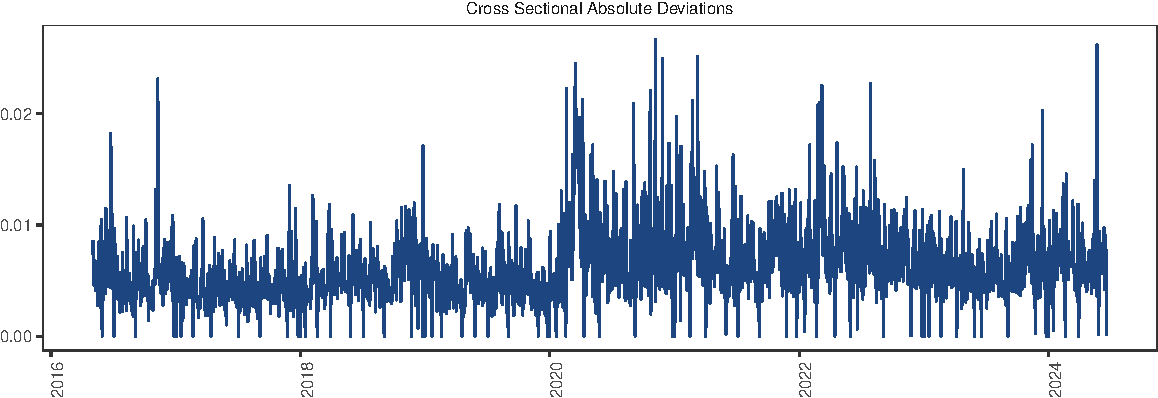
\includegraphics{alt_energy_herding_files/figure-pdf/fig-csad-1.pdf}

}

\caption{\label{fig-csad}Cross Sectional Absolute Deviation (CSAD) for
US Alternative Energy ETFs}

\end{figure}%

The development of the CSAD measure over time for the clean energy ETFs
is presented in Figure~\ref{fig-csad}. In general, the CSAD measure
remains within certain bounds. However, we observe several cases when
the CSAD measure deviates significantly from the market consensus:
around the announcement of the Paris agreement (2016-2017), the covid-19
pandemic crisis (2020--2021), the war outbreak in Ukraine (2022) among
others. Table~\ref{tbl-desc} presents the descriptive statistics of the
data.

\global\setlength{\Oldarrayrulewidth}{\arrayrulewidth}

\global\setlength{\Oldtabcolsep}{\tabcolsep}

\setlength{\tabcolsep}{2pt}

\renewcommand*{\arraystretch}{0.7}



\providecommand{\ascline}[3]{\noalign{\global\arrayrulewidth #1}\arrayrulecolor[HTML]{#2}\cline{#3}}

\begin{longtable}[l]{|p{1.46in}|p{1.08in}|p{1.08in}|p{1.23in}|p{1.14in}}

\caption{\label{tbl-desc}Descriptive statistics of the data}

\tabularnewline

\ascline{1pt}{000000}{1-5}

\multicolumn{1}{!{\color[HTML]{FFFFFF}\vrule width 1pt}>{\raggedright}m{\dimexpr 1.46in+0\tabcolsep}}{\textcolor[HTML]{000000}{\fontsize{7}{7}\selectfont{\global\setmainfont{Arial}{\ }}}} & \multicolumn{1}{!{\color[HTML]{FFFFFF}\vrule width 1pt}>{\centering}m{\dimexpr 1.08in+0\tabcolsep}}{\textcolor[HTML]{000000}{\fontsize{7}{7}\selectfont{\global\setmainfont{Arial}{Mean}}}} & \multicolumn{1}{!{\color[HTML]{FFFFFF}\vrule width 1pt}>{\centering}m{\dimexpr 1.08in+0\tabcolsep}}{\textcolor[HTML]{000000}{\fontsize{7}{7}\selectfont{\global\setmainfont{Arial}{St.dev}}}} & \multicolumn{1}{!{\color[HTML]{FFFFFF}\vrule width 1pt}>{\centering}m{\dimexpr 1.23in+0\tabcolsep}}{\textcolor[HTML]{000000}{\fontsize{7}{7}\selectfont{\global\setmainfont{Arial}{Skewness}}}} & \multicolumn{1}{!{\color[HTML]{FFFFFF}\vrule width 1pt}>{\centering}m{\dimexpr 1.14in+0\tabcolsep}!{\color[HTML]{FFFFFF}\vrule width 1pt}}{\textcolor[HTML]{000000}{\fontsize{7}{7}\selectfont{\global\setmainfont{Arial}{Kurtosis}}}} \\

\ascline{1pt}{000000}{1-5}\endfirsthead 

\ascline{1pt}{000000}{1-5}

\multicolumn{1}{!{\color[HTML]{FFFFFF}\vrule width 1pt}>{\raggedright}m{\dimexpr 1.46in+0\tabcolsep}}{\textcolor[HTML]{000000}{\fontsize{7}{7}\selectfont{\global\setmainfont{Arial}{\ }}}} & \multicolumn{1}{!{\color[HTML]{FFFFFF}\vrule width 1pt}>{\centering}m{\dimexpr 1.08in+0\tabcolsep}}{\textcolor[HTML]{000000}{\fontsize{7}{7}\selectfont{\global\setmainfont{Arial}{Mean}}}} & \multicolumn{1}{!{\color[HTML]{FFFFFF}\vrule width 1pt}>{\centering}m{\dimexpr 1.08in+0\tabcolsep}}{\textcolor[HTML]{000000}{\fontsize{7}{7}\selectfont{\global\setmainfont{Arial}{St.dev}}}} & \multicolumn{1}{!{\color[HTML]{FFFFFF}\vrule width 1pt}>{\centering}m{\dimexpr 1.23in+0\tabcolsep}}{\textcolor[HTML]{000000}{\fontsize{7}{7}\selectfont{\global\setmainfont{Arial}{Skewness}}}} & \multicolumn{1}{!{\color[HTML]{FFFFFF}\vrule width 1pt}>{\centering}m{\dimexpr 1.14in+0\tabcolsep}!{\color[HTML]{FFFFFF}\vrule width 1pt}}{\textcolor[HTML]{000000}{\fontsize{7}{7}\selectfont{\global\setmainfont{Arial}{Kurtosis}}}} \\

\ascline{1pt}{000000}{1-5}\endhead



\multicolumn{1}{!{\color[HTML]{FFFFFF}\vrule width 1pt}>{\raggedright}m{\dimexpr 1.46in+0\tabcolsep}}{\textcolor[HTML]{000000}{\fontsize{7}{7}\selectfont{\global\setmainfont{Arial}{CSAD}}}} & \multicolumn{1}{!{\color[HTML]{FFFFFF}\vrule width 1pt}>{\centering}m{\dimexpr 1.08in+0\tabcolsep}}{\textcolor[HTML]{000000}{\fontsize{7}{7}\selectfont{\global\setmainfont{Arial}{0.0062}}}} & \multicolumn{1}{!{\color[HTML]{FFFFFF}\vrule width 1pt}>{\centering}m{\dimexpr 1.08in+0\tabcolsep}}{\textcolor[HTML]{000000}{\fontsize{7}{7}\selectfont{\global\setmainfont{Arial}{0.0034}}}} & \multicolumn{1}{!{\color[HTML]{FFFFFF}\vrule width 1pt}>{\centering}m{\dimexpr 1.23in+0\tabcolsep}}{\textcolor[HTML]{000000}{\fontsize{7}{7}\selectfont{\global\setmainfont{Arial}{1.5598}}}} & \multicolumn{1}{!{\color[HTML]{FFFFFF}\vrule width 1pt}>{\centering}m{\dimexpr 1.14in+0\tabcolsep}!{\color[HTML]{FFFFFF}\vrule width 1pt}}{\textcolor[HTML]{000000}{\fontsize{7}{7}\selectfont{\global\setmainfont{Arial}{7.9355}}}} \\

\ascline{1pt}{FFFFFF}{1-5}



\multicolumn{1}{!{\color[HTML]{FFFFFF}\vrule width 1pt}>{\raggedright}m{\dimexpr 1.46in+0\tabcolsep}}{\textcolor[HTML]{000000}{\fontsize{7}{7}\selectfont{\global\setmainfont{Arial}{Absolute\ CSAR}}}} & \multicolumn{1}{!{\color[HTML]{FFFFFF}\vrule width 1pt}>{\centering}m{\dimexpr 1.08in+0\tabcolsep}}{\textcolor[HTML]{000000}{\fontsize{7}{7}\selectfont{\global\setmainfont{Arial}{0.0094}}}} & \multicolumn{1}{!{\color[HTML]{FFFFFF}\vrule width 1pt}>{\centering}m{\dimexpr 1.08in+0\tabcolsep}}{\textcolor[HTML]{000000}{\fontsize{7}{7}\selectfont{\global\setmainfont{Arial}{0.0107}}}} & \multicolumn{1}{!{\color[HTML]{FFFFFF}\vrule width 1pt}>{\centering}m{\dimexpr 1.23in+0\tabcolsep}}{\textcolor[HTML]{000000}{\fontsize{7}{7}\selectfont{\global\setmainfont{Arial}{3.3175}}}} & \multicolumn{1}{!{\color[HTML]{FFFFFF}\vrule width 1pt}>{\centering}m{\dimexpr 1.14in+0\tabcolsep}!{\color[HTML]{FFFFFF}\vrule width 1pt}}{\textcolor[HTML]{000000}{\fontsize{7}{7}\selectfont{\global\setmainfont{Arial}{23.8725}}}} \\

\ascline{1pt}{000000}{1-5}


\end{longtable}

\arrayrulecolor[HTML]{000000}

\global\setlength{\arrayrulewidth}{\Oldarrayrulewidth}

\global\setlength{\tabcolsep}{\Oldtabcolsep}

\renewcommand*{\arraystretch}{1}

\subsection{Methodology}\label{methodology}

Following the relevant literature
\citetext{\citealp{christie1995}; \citealp[and][]{chang2000}}, we
compute dispersion of the \(i^{th}\) ETF from the market return. This is
known as the Cross Sectional Absolute Deviation (\(CSAD_t\)) measure.
Empirically the \(CSAD_t\) is defined in the following manner:

\begin{equation}\phantomsection\label{eq-csad}{
CSAD_t = \dfrac{1}{N}\sum_{i=1}^{N} |R_{i,t} - R_{m,t}|,
}\end{equation}

where \(R_{i,t}\) is the return and \(R_{m,t}\) is the cross sectional
average of returns for the sample of ETFs available for each day. The
return dispersion measures the directional similarity of ETF returns to
the market return. This return similarity forms the basis for the
herding behaviour tests. Following \citet{galariotis2015} we estimate
Equation~\ref{eq-herding}:

\begin{equation}\phantomsection\label{eq-herding}{
CSAD_t = \gamma_0 + \gamma_1 |R_{m,t}| + \gamma_2 R_{m,t}^2 + \epsilon_t,
}\end{equation}

where \(\gamma_0\) is the intercept, \(\gamma_1\) is the coefficient of
the linear term, \(\gamma_2\) is the coefficient of the quadratic term
or the herding behaviour term, and \(\epsilon_t\) is the error term. The
coefficient \(\gamma_2 <0\) when herding is present, and \(\gamma_2 >0\)
when anti-herding is present. To ensure the robustness of the estimate,
we estimate \(CSAD_{t}\) with Newey-West standard errors
\citep[See][]{newey1987}.

Based on the above and in order to provide additional insight on the
herding phenomenon we examine whether herding presents an asymmetric
response on days when the market is up vis-à-vis days when the market is
down. To this end, we augment Equation~\ref{eq-herding} as follows:

\begin{equation}\phantomsection\label{eq-asymmetry}{
CSAD_t = \gamma_0 + \gamma_1(1-D) R_{m,t} + \gamma_2D R_{m,t} + \gamma_3(1-D) R_{m,t}^2  + \gamma_4D R_{m,t}^2 + \epsilon_t,
}\end{equation}

where \(D\) is a dummy variable that takes the value of 1 when the
market return is negative and 0 otherwise. Therefore, our exploration of
asymmetric behaviour of herding phenomenon is carried through the
inspection of the statistical significance and the sign of the two
estimated coefficients \(\gamma_3\) versus \(\gamma_4\) (up versus down
markets).

\section{Results}\label{results}

\subsection{Herding behaviour}\label{herding-behaviour}

Rational asset pricing models \citep[for example,][]{black1972} predict
a linear relationship between return dispersion and market returns under
normal conditions, a relationship that is no longer valid in the
presence of herding. Herding behaviour leads to an increasing or
decreasing cross sectional dispersion with respect to market returns. In
other words, herding is captured by a non-linear term in the standard
pricing equation indicating a decreasing or an increasing returns'
dispersion.

Stated differently, as \citet{chang2000} argue, in the case of herding
the coefficient on the non-linear term (\(\gamma_2\)) will be negative
and statistically significant. Table~\ref{tbl-herding} presents the
results of herding for the full sample employing the non-linear
Equation~\ref{eq-herding}. The estimated coefficient on market return is
positive and highly significant as expected. The estimated coefficient
on the non-linear term is negative (-1.2773) and statistically
significant with a t-statistic of -9.71 suggesting that herd behaviour
is present and robust in the US alternative energy ETFs.

\global\setlength{\Oldarrayrulewidth}{\arrayrulewidth}

\global\setlength{\Oldtabcolsep}{\tabcolsep}

\setlength{\tabcolsep}{2pt}

\renewcommand*{\arraystretch}{0.9}



\providecommand{\ascline}[3]{\noalign{\global\arrayrulewidth #1}\arrayrulecolor[HTML]{#2}\cline{#3}}

\begin{longtable}[l]{|p{1.99in}|p{1.99in}|p{1.99in}}

\caption{\label{tbl-herding}Estimation results of herding in the U.S.
equity alternative energy ETFs}

\tabularnewline

\ascline{1pt}{000000}{1-3}

\multicolumn{1}{!{\color[HTML]{FFFFFF}\vrule width 1pt}>{\centering}m{\dimexpr 1.99in+0\tabcolsep}}{\textcolor[HTML]{000000}{\fontsize{7}{7}\selectfont{\global\setmainfont{Arial}{$\gamma_0$}}}} & \multicolumn{1}{!{\color[HTML]{FFFFFF}\vrule width 1pt}>{\centering}m{\dimexpr 1.99in+0\tabcolsep}}{\textcolor[HTML]{000000}{\fontsize{7}{7}\selectfont{\global\setmainfont{Arial}{$\gamma_1 $}}}} & \multicolumn{1}{!{\color[HTML]{FFFFFF}\vrule width 1pt}>{\centering}m{\dimexpr 1.99in+0\tabcolsep}!{\color[HTML]{FFFFFF}\vrule width 1pt}}{\textcolor[HTML]{000000}{\fontsize{7}{7}\selectfont{\global\setmainfont{Arial}{$\gamma_2$}}}} \\

\ascline{1pt}{000000}{1-3}\endfirsthead 

\ascline{1pt}{000000}{1-3}

\multicolumn{1}{!{\color[HTML]{FFFFFF}\vrule width 1pt}>{\centering}m{\dimexpr 1.99in+0\tabcolsep}}{\textcolor[HTML]{000000}{\fontsize{7}{7}\selectfont{\global\setmainfont{Arial}{$\gamma_0$}}}} & \multicolumn{1}{!{\color[HTML]{FFFFFF}\vrule width 1pt}>{\centering}m{\dimexpr 1.99in+0\tabcolsep}}{\textcolor[HTML]{000000}{\fontsize{7}{7}\selectfont{\global\setmainfont{Arial}{$\gamma_1 $}}}} & \multicolumn{1}{!{\color[HTML]{FFFFFF}\vrule width 1pt}>{\centering}m{\dimexpr 1.99in+0\tabcolsep}!{\color[HTML]{FFFFFF}\vrule width 1pt}}{\textcolor[HTML]{000000}{\fontsize{7}{7}\selectfont{\global\setmainfont{Arial}{$\gamma_2$}}}} \\

\ascline{1pt}{000000}{1-3}\endhead



\multicolumn{1}{!{\color[HTML]{FFFFFF}\vrule width 1pt}>{\centering}m{\dimexpr 1.99in+0\tabcolsep}}{\textcolor[HTML]{000000}{\fontsize{7}{7}\selectfont{\global\setmainfont{Arial}{0.0038**}}}} & \multicolumn{1}{!{\color[HTML]{FFFFFF}\vrule width 1pt}>{\centering}m{\dimexpr 1.99in+0\tabcolsep}}{\textcolor[HTML]{000000}{\fontsize{7}{7}\selectfont{\global\setmainfont{Arial}{0.2883***}}}} & \multicolumn{1}{!{\color[HTML]{FFFFFF}\vrule width 1pt}>{\centering}m{\dimexpr 1.99in+0\tabcolsep}!{\color[HTML]{FFFFFF}\vrule width 1pt}}{\textcolor[HTML]{000000}{\fontsize{7}{7}\selectfont{\global\setmainfont{Arial}{\ -1.2773***}}}} \\

\ascline{1pt}{FFFFFF}{1-3}



\multicolumn{1}{!{\color[HTML]{FFFFFF}\vrule width 1pt}>{\centering}m{\dimexpr 1.99in+0\tabcolsep}}{\textcolor[HTML]{000000}{\fontsize{7}{7}\selectfont{\global\setmainfont{Arial}{(47.09)}}}} & \multicolumn{1}{!{\color[HTML]{FFFFFF}\vrule width 1pt}>{\centering}m{\dimexpr 1.99in+0\tabcolsep}}{\textcolor[HTML]{000000}{\fontsize{7}{7}\selectfont{\global\setmainfont{Arial}{(33.333)}}}} & \multicolumn{1}{!{\color[HTML]{FFFFFF}\vrule width 1pt}>{\centering}m{\dimexpr 1.99in+0\tabcolsep}!{\color[HTML]{FFFFFF}\vrule width 1pt}}{\textcolor[HTML]{000000}{\fontsize{7}{7}\selectfont{\global\setmainfont{Arial}{(-9.71)}}}} \\

\ascline{1pt}{000000}{1-3}



\multicolumn{3}{>{\raggedright}m{\dimexpr 5.96in+4\tabcolsep}}{\textcolor[HTML]{000000}{\fontsize{7}{7}\selectfont{\global\setmainfont{Arial}{Note:\ *,**,***\ denotes\ significance\ at\ 10\%,5\%\ and\ 1\%\ respectively.}}}} \\

\ascline{1pt}{000000}{1-3}


\end{longtable}

\arrayrulecolor[HTML]{000000}

\global\setlength{\arrayrulewidth}{\Oldarrayrulewidth}

\global\setlength{\tabcolsep}{\Oldtabcolsep}

\renewcommand*{\arraystretch}{1}

There is ample evidence in the relevant literature that herding
behaviour in various asset markets \citep[see][]{pochea2017} exhibits
asymmetry and time-varying characteristics. To this end, we proceed to
estimate Equation~\ref{eq-herding} using the quantile regression (QR)
proposed by \citet{koenker1978}. Table~\ref{tbl-quantile_herding}
presents the results of estimating Equation~\ref{eq-herding} across
various quantiles of the returns dispersion. Our focus is on the herding
coefficient \(\gamma_2\), as a significant negative value of
\(\gamma_2\) is indicative of herding. Such a finding is observed at two
quantiles namely 25\% and 50\% with a value of -1.1056 and -1.165 which
are highly significant. It is worth mentioning that the sign of the
herding coefficient remains negative for almost all quantiles while the
significance changes from significant to insignificant while we move
from low and middle to upper quantiles (75\% and 90\%).

\global\setlength{\Oldarrayrulewidth}{\arrayrulewidth}

\global\setlength{\Oldtabcolsep}{\tabcolsep}

\setlength{\tabcolsep}{2pt}

\renewcommand*{\arraystretch}{0.7}



\providecommand{\ascline}[3]{\noalign{\global\arrayrulewidth #1}\arrayrulecolor[HTML]{#2}\cline{#3}}

\begin{longtable}[l]{|p{1.49in}|p{1.49in}|p{1.49in}|p{1.49in}}

\caption{\label{tbl-quantile_herding}Estimation results of herding
across various quantiles}

\tabularnewline

\ascline{1pt}{000000}{1-4}

\multicolumn{1}{!{\color[HTML]{FFFFFF}\vrule width 1pt}>{\centering}m{\dimexpr 1.49in+0\tabcolsep}}{\textcolor[HTML]{000000}{\fontsize{7}{7}\selectfont{\global\setmainfont{Arial}{Quantile}}}} & \multicolumn{1}{!{\color[HTML]{FFFFFF}\vrule width 1pt}>{\centering}m{\dimexpr 1.49in+0\tabcolsep}}{\textcolor[HTML]{000000}{\fontsize{7}{7}\selectfont{\global\setmainfont{Arial}{$\gamma_0$}}}} & \multicolumn{1}{!{\color[HTML]{FFFFFF}\vrule width 1pt}>{\centering}m{\dimexpr 1.49in+0\tabcolsep}}{\textcolor[HTML]{000000}{\fontsize{7}{7}\selectfont{\global\setmainfont{Arial}{$\gamma_1 $}}}} & \multicolumn{1}{!{\color[HTML]{FFFFFF}\vrule width 1pt}>{\centering}m{\dimexpr 1.49in+0\tabcolsep}!{\color[HTML]{FFFFFF}\vrule width 1pt}}{\textcolor[HTML]{000000}{\fontsize{7}{7}\selectfont{\global\setmainfont{Arial}{$\gamma_2$}}}} \\

\ascline{1pt}{000000}{1-4}\endfirsthead 

\ascline{1pt}{000000}{1-4}

\multicolumn{1}{!{\color[HTML]{FFFFFF}\vrule width 1pt}>{\centering}m{\dimexpr 1.49in+0\tabcolsep}}{\textcolor[HTML]{000000}{\fontsize{7}{7}\selectfont{\global\setmainfont{Arial}{Quantile}}}} & \multicolumn{1}{!{\color[HTML]{FFFFFF}\vrule width 1pt}>{\centering}m{\dimexpr 1.49in+0\tabcolsep}}{\textcolor[HTML]{000000}{\fontsize{7}{7}\selectfont{\global\setmainfont{Arial}{$\gamma_0$}}}} & \multicolumn{1}{!{\color[HTML]{FFFFFF}\vrule width 1pt}>{\centering}m{\dimexpr 1.49in+0\tabcolsep}}{\textcolor[HTML]{000000}{\fontsize{7}{7}\selectfont{\global\setmainfont{Arial}{$\gamma_1 $}}}} & \multicolumn{1}{!{\color[HTML]{FFFFFF}\vrule width 1pt}>{\centering}m{\dimexpr 1.49in+0\tabcolsep}!{\color[HTML]{FFFFFF}\vrule width 1pt}}{\textcolor[HTML]{000000}{\fontsize{7}{7}\selectfont{\global\setmainfont{Arial}{$\gamma_2$}}}} \\

\ascline{1pt}{000000}{1-4}\endhead



\multicolumn{1}{!{\color[HTML]{FFFFFF}\vrule width 1pt}>{\centering}m{\dimexpr 1.49in+0\tabcolsep}}{\textcolor[HTML]{000000}{\fontsize{7}{7}\selectfont{\global\setmainfont{Arial}{$\tau = 10\%$}}}} & \multicolumn{1}{!{\color[HTML]{FFFFFF}\vrule width 1pt}>{\centering}m{\dimexpr 1.49in+0\tabcolsep}}{\textcolor[HTML]{000000}{\fontsize{7}{7}\selectfont{\global\setmainfont{Arial}{0.0016***}}}} & \multicolumn{1}{!{\color[HTML]{FFFFFF}\vrule width 1pt}>{\centering}m{\dimexpr 1.49in+0\tabcolsep}}{\textcolor[HTML]{000000}{\fontsize{7}{7}\selectfont{\global\setmainfont{Arial}{0.2536***}}}} & \multicolumn{1}{!{\color[HTML]{FFFFFF}\vrule width 1pt}>{\centering}m{\dimexpr 1.49in+0\tabcolsep}!{\color[HTML]{FFFFFF}\vrule width 1pt}}{\textcolor[HTML]{000000}{\fontsize{7}{7}\selectfont{\global\setmainfont{Arial}{\ -1.3736}}}} \\

\ascline{1pt}{FFFFFF}{1-4}



\multicolumn{1}{!{\color[HTML]{FFFFFF}\vrule width 1pt}>{\centering}m{\dimexpr 1.49in+0\tabcolsep}}{\textcolor[HTML]{000000}{\fontsize{7}{7}\selectfont{\global\setmainfont{Arial}{$\tau = 25\%$}}}} & \multicolumn{1}{!{\color[HTML]{FFFFFF}\vrule width 1pt}>{\centering}m{\dimexpr 1.49in+0\tabcolsep}}{\textcolor[HTML]{000000}{\fontsize{7}{7}\selectfont{\global\setmainfont{Arial}{0.0026***}}}} & \multicolumn{1}{!{\color[HTML]{FFFFFF}\vrule width 1pt}>{\centering}m{\dimexpr 1.49in+0\tabcolsep}}{\textcolor[HTML]{000000}{\fontsize{7}{7}\selectfont{\global\setmainfont{Arial}{0.2461***}}}} & \multicolumn{1}{!{\color[HTML]{FFFFFF}\vrule width 1pt}>{\centering}m{\dimexpr 1.49in+0\tabcolsep}!{\color[HTML]{FFFFFF}\vrule width 1pt}}{\textcolor[HTML]{000000}{\fontsize{7}{7}\selectfont{\global\setmainfont{Arial}{\ -1.1056***}}}} \\

\ascline{1pt}{FFFFFF}{1-4}



\multicolumn{1}{!{\color[HTML]{FFFFFF}\vrule width 1pt}>{\centering}m{\dimexpr 1.49in+0\tabcolsep}}{\textcolor[HTML]{000000}{\fontsize{7}{7}\selectfont{\global\setmainfont{Arial}{$\tau = 50\%$}}}} & \multicolumn{1}{!{\color[HTML]{FFFFFF}\vrule width 1pt}>{\centering}m{\dimexpr 1.49in+0\tabcolsep}}{\textcolor[HTML]{000000}{\fontsize{7}{7}\selectfont{\global\setmainfont{Arial}{0.0037***}}}} & \multicolumn{1}{!{\color[HTML]{FFFFFF}\vrule width 1pt}>{\centering}m{\dimexpr 1.49in+0\tabcolsep}}{\textcolor[HTML]{000000}{\fontsize{7}{7}\selectfont{\global\setmainfont{Arial}{0.2648***}}}} & \multicolumn{1}{!{\color[HTML]{FFFFFF}\vrule width 1pt}>{\centering}m{\dimexpr 1.49in+0\tabcolsep}!{\color[HTML]{FFFFFF}\vrule width 1pt}}{\textcolor[HTML]{000000}{\fontsize{7}{7}\selectfont{\global\setmainfont{Arial}{\ -1.165***}}}} \\

\ascline{1pt}{FFFFFF}{1-4}



\multicolumn{1}{!{\color[HTML]{FFFFFF}\vrule width 1pt}>{\centering}m{\dimexpr 1.49in+0\tabcolsep}}{\textcolor[HTML]{000000}{\fontsize{7}{7}\selectfont{\global\setmainfont{Arial}{$\tau = 75\%$}}}} & \multicolumn{1}{!{\color[HTML]{FFFFFF}\vrule width 1pt}>{\centering}m{\dimexpr 1.49in+0\tabcolsep}}{\textcolor[HTML]{000000}{\fontsize{7}{7}\selectfont{\global\setmainfont{Arial}{0.0048***}}}} & \multicolumn{1}{!{\color[HTML]{FFFFFF}\vrule width 1pt}>{\centering}m{\dimexpr 1.49in+0\tabcolsep}}{\textcolor[HTML]{000000}{\fontsize{7}{7}\selectfont{\global\setmainfont{Arial}{0.3011***}}}} & \multicolumn{1}{!{\color[HTML]{FFFFFF}\vrule width 1pt}>{\centering}m{\dimexpr 1.49in+0\tabcolsep}!{\color[HTML]{FFFFFF}\vrule width 1pt}}{\textcolor[HTML]{000000}{\fontsize{7}{7}\selectfont{\global\setmainfont{Arial}{\ -1.1473***}}}} \\

\ascline{1pt}{FFFFFF}{1-4}



\multicolumn{1}{!{\color[HTML]{FFFFFF}\vrule width 1pt}>{\centering}m{\dimexpr 1.49in+0\tabcolsep}}{\textcolor[HTML]{000000}{\fontsize{7}{7}\selectfont{\global\setmainfont{Arial}{$\tau = 90\%$}}}} & \multicolumn{1}{!{\color[HTML]{FFFFFF}\vrule width 1pt}>{\centering}m{\dimexpr 1.49in+0\tabcolsep}}{\textcolor[HTML]{000000}{\fontsize{7}{7}\selectfont{\global\setmainfont{Arial}{0.0064***}}}} & \multicolumn{1}{!{\color[HTML]{FFFFFF}\vrule width 1pt}>{\centering}m{\dimexpr 1.49in+0\tabcolsep}}{\textcolor[HTML]{000000}{\fontsize{7}{7}\selectfont{\global\setmainfont{Arial}{0.2999***}}}} & \multicolumn{1}{!{\color[HTML]{FFFFFF}\vrule width 1pt}>{\centering}m{\dimexpr 1.49in+0\tabcolsep}!{\color[HTML]{FFFFFF}\vrule width 1pt}}{\textcolor[HTML]{000000}{\fontsize{7}{7}\selectfont{\global\setmainfont{Arial}{\ 0.2314}}}} \\

\ascline{1pt}{000000}{1-4}



\multicolumn{4}{>{\raggedright}m{\dimexpr 5.94in+6\tabcolsep}}{\textcolor[HTML]{000000}{\fontsize{7}{7}\selectfont{\global\setmainfont{Arial}{Note:\ This\ table\ presents\ the\ estimation\ results\ of\ herding\ of\ US\ Alternative\ energy\ equity\ ETFs\ according\ to\ Equation\ 2\ in\ various\ quantiles\ 10,\ 25,\ 50,\ 75\ and\ 90\%\ of\ the\ returns\ distribution.}}}\textcolor[HTML]{000000}{\fontsize{7}{7}\selectfont{\global\setmainfont{Arial}{\ }}}\textcolor[HTML]{000000}{\fontsize{7}{7}\selectfont{\global\setmainfont{Arial}{*,**,***\ denotes\ significance\ at\ 10\%,5\%\ and\ 1\%\ respectively.}}}} \\

\ascline{1pt}{000000}{1-4}


\end{longtable}

\arrayrulecolor[HTML]{000000}

\global\setlength{\arrayrulewidth}{\Oldarrayrulewidth}

\global\setlength{\tabcolsep}{\Oldtabcolsep}

\renewcommand*{\arraystretch}{1}

\subsection{Herding behaviour during extreme market
periods}\label{herding-behaviour-during-extreme-market-periods}

It is widely accepted that asset returns are characterized by asymmetry,
that is, return dispersion tend to behave differently in rising and
falling markets \citep[see][]{geert2000, zhou2013, longin2001}. It
should be noted, that examining the relationship between returns
dispersion and market-wide returns across various quantiles of the
returns distribution allows us to make more robust inference regarding
the true behaviour of the phenomenon. Table~\ref{tbl-asymmetry_herding}
reports the estimation results of herding in the up and down markets
based on Equation~\ref{eq-asymmetry}. In general, we find that herding
is more likely to occur in down markets than in up markets, which is
indicative of the asymmetry of herding behaviour.

\newpage

\global\setlength{\Oldarrayrulewidth}{\arrayrulewidth}

\global\setlength{\Oldtabcolsep}{\tabcolsep}

\setlength{\tabcolsep}{2pt}

\renewcommand*{\arraystretch}{0.7}



\providecommand{\ascline}[3]{\noalign{\global\arrayrulewidth #1}\arrayrulecolor[HTML]{#2}\cline{#3}}

\begin{longtable}[l]{|p{0.99in}|p{0.99in}|p{0.99in}|p{0.99in}|p{0.99in}|p{0.99in}}

\caption{\label{tbl-asymmetry_herding}Estimation results of herding in
up and down markets}

\tabularnewline

\ascline{1pt}{000000}{1-6}

\multicolumn{1}{!{\color[HTML]{FFFFFF}\vrule width 1pt}>{\centering}m{\dimexpr 0.99in+0\tabcolsep}}{\textcolor[HTML]{000000}{\fontsize{7}{7}\selectfont{\global\setmainfont{Arial}{Quantile}}}} & \multicolumn{1}{!{\color[HTML]{FFFFFF}\vrule width 1pt}>{\centering}m{\dimexpr 0.99in+0\tabcolsep}}{\textcolor[HTML]{000000}{\fontsize{7}{7}\selectfont{\global\setmainfont{Arial}{$\gamma_0$}}}} & \multicolumn{1}{!{\color[HTML]{FFFFFF}\vrule width 1pt}>{\centering}m{\dimexpr 0.99in+0\tabcolsep}}{\textcolor[HTML]{000000}{\fontsize{7}{7}\selectfont{\global\setmainfont{Arial}{$\gamma_1 $}}}} & \multicolumn{1}{!{\color[HTML]{FFFFFF}\vrule width 1pt}>{\centering}m{\dimexpr 0.99in+0\tabcolsep}}{\textcolor[HTML]{000000}{\fontsize{7}{7}\selectfont{\global\setmainfont{Arial}{$\gamma_2$}}}} & \multicolumn{1}{!{\color[HTML]{FFFFFF}\vrule width 1pt}>{\centering}m{\dimexpr 0.99in+0\tabcolsep}}{\textcolor[HTML]{000000}{\fontsize{7}{7}\selectfont{\global\setmainfont{Arial}{$\gamma_3$}}}} & \multicolumn{1}{!{\color[HTML]{FFFFFF}\vrule width 1pt}>{\centering}m{\dimexpr 0.99in+0\tabcolsep}!{\color[HTML]{FFFFFF}\vrule width 1pt}}{\textcolor[HTML]{000000}{\fontsize{7}{7}\selectfont{\global\setmainfont{Arial}{$\gamma_4$}}}} \\

\ascline{1pt}{000000}{1-6}\endfirsthead 

\ascline{1pt}{000000}{1-6}

\multicolumn{1}{!{\color[HTML]{FFFFFF}\vrule width 1pt}>{\centering}m{\dimexpr 0.99in+0\tabcolsep}}{\textcolor[HTML]{000000}{\fontsize{7}{7}\selectfont{\global\setmainfont{Arial}{Quantile}}}} & \multicolumn{1}{!{\color[HTML]{FFFFFF}\vrule width 1pt}>{\centering}m{\dimexpr 0.99in+0\tabcolsep}}{\textcolor[HTML]{000000}{\fontsize{7}{7}\selectfont{\global\setmainfont{Arial}{$\gamma_0$}}}} & \multicolumn{1}{!{\color[HTML]{FFFFFF}\vrule width 1pt}>{\centering}m{\dimexpr 0.99in+0\tabcolsep}}{\textcolor[HTML]{000000}{\fontsize{7}{7}\selectfont{\global\setmainfont{Arial}{$\gamma_1 $}}}} & \multicolumn{1}{!{\color[HTML]{FFFFFF}\vrule width 1pt}>{\centering}m{\dimexpr 0.99in+0\tabcolsep}}{\textcolor[HTML]{000000}{\fontsize{7}{7}\selectfont{\global\setmainfont{Arial}{$\gamma_2$}}}} & \multicolumn{1}{!{\color[HTML]{FFFFFF}\vrule width 1pt}>{\centering}m{\dimexpr 0.99in+0\tabcolsep}}{\textcolor[HTML]{000000}{\fontsize{7}{7}\selectfont{\global\setmainfont{Arial}{$\gamma_3$}}}} & \multicolumn{1}{!{\color[HTML]{FFFFFF}\vrule width 1pt}>{\centering}m{\dimexpr 0.99in+0\tabcolsep}!{\color[HTML]{FFFFFF}\vrule width 1pt}}{\textcolor[HTML]{000000}{\fontsize{7}{7}\selectfont{\global\setmainfont{Arial}{$\gamma_4$}}}} \\

\ascline{1pt}{000000}{1-6}\endhead



\multicolumn{1}{!{\color[HTML]{FFFFFF}\vrule width 1pt}>{\centering}m{\dimexpr 0.99in+0\tabcolsep}}{\textcolor[HTML]{000000}{\fontsize{7}{7}\selectfont{\global\setmainfont{Arial}{$\tau = 10\%$}}}} & \multicolumn{1}{!{\color[HTML]{FFFFFF}\vrule width 1pt}>{\centering}m{\dimexpr 0.99in+0\tabcolsep}}{\textcolor[HTML]{000000}{\fontsize{7}{7}\selectfont{\global\setmainfont{Arial}{0.0016***}}}} & \multicolumn{1}{!{\color[HTML]{FFFFFF}\vrule width 1pt}>{\centering}m{\dimexpr 0.99in+0\tabcolsep}}{\textcolor[HTML]{000000}{\fontsize{7}{7}\selectfont{\global\setmainfont{Arial}{0.2532***}}}} & \multicolumn{1}{!{\color[HTML]{FFFFFF}\vrule width 1pt}>{\centering}m{\dimexpr 0.99in+0\tabcolsep}}{\textcolor[HTML]{000000}{\fontsize{7}{7}\selectfont{\global\setmainfont{Arial}{\ -1.3669***}}}} & \multicolumn{1}{!{\color[HTML]{FFFFFF}\vrule width 1pt}>{\centering}m{\dimexpr 0.99in+0\tabcolsep}}{\textcolor[HTML]{000000}{\fontsize{7}{7}\selectfont{\global\setmainfont{Arial}{\ -0.2522***}}}} & \multicolumn{1}{!{\color[HTML]{FFFFFF}\vrule width 1pt}>{\centering}m{\dimexpr 0.99in+0\tabcolsep}!{\color[HTML]{FFFFFF}\vrule width 1pt}}{\textcolor[HTML]{000000}{\fontsize{7}{7}\selectfont{\global\setmainfont{Arial}{\ -1.1522}}}} \\

\ascline{1pt}{FFFFFF}{1-6}



\multicolumn{1}{!{\color[HTML]{FFFFFF}\vrule width 1pt}>{\centering}m{\dimexpr 0.99in+0\tabcolsep}}{\textcolor[HTML]{000000}{\fontsize{7}{7}\selectfont{\global\setmainfont{Arial}{$\tau = 25\%$}}}} & \multicolumn{1}{!{\color[HTML]{FFFFFF}\vrule width 1pt}>{\centering}m{\dimexpr 0.99in+0\tabcolsep}}{\textcolor[HTML]{000000}{\fontsize{7}{7}\selectfont{\global\setmainfont{Arial}{0.0026***}}}} & \multicolumn{1}{!{\color[HTML]{FFFFFF}\vrule width 1pt}>{\centering}m{\dimexpr 0.99in+0\tabcolsep}}{\textcolor[HTML]{000000}{\fontsize{7}{7}\selectfont{\global\setmainfont{Arial}{0.2475***}}}} & \multicolumn{1}{!{\color[HTML]{FFFFFF}\vrule width 1pt}>{\centering}m{\dimexpr 0.99in+0\tabcolsep}}{\textcolor[HTML]{000000}{\fontsize{7}{7}\selectfont{\global\setmainfont{Arial}{\ -1.2383**}}}} & \multicolumn{1}{!{\color[HTML]{FFFFFF}\vrule width 1pt}>{\centering}m{\dimexpr 0.99in+0\tabcolsep}}{\textcolor[HTML]{000000}{\fontsize{7}{7}\selectfont{\global\setmainfont{Arial}{\ -0.2477***}}}} & \multicolumn{1}{!{\color[HTML]{FFFFFF}\vrule width 1pt}>{\centering}m{\dimexpr 0.99in+0\tabcolsep}!{\color[HTML]{FFFFFF}\vrule width 1pt}}{\textcolor[HTML]{000000}{\fontsize{7}{7}\selectfont{\global\setmainfont{Arial}{\ -1.1171***}}}} \\

\ascline{1pt}{FFFFFF}{1-6}



\multicolumn{1}{!{\color[HTML]{FFFFFF}\vrule width 1pt}>{\centering}m{\dimexpr 0.99in+0\tabcolsep}}{\textcolor[HTML]{000000}{\fontsize{7}{7}\selectfont{\global\setmainfont{Arial}{$\tau = 50\%$}}}} & \multicolumn{1}{!{\color[HTML]{FFFFFF}\vrule width 1pt}>{\centering}m{\dimexpr 0.99in+0\tabcolsep}}{\textcolor[HTML]{000000}{\fontsize{7}{7}\selectfont{\global\setmainfont{Arial}{0.0038***}}}} & \multicolumn{1}{!{\color[HTML]{FFFFFF}\vrule width 1pt}>{\centering}m{\dimexpr 0.99in+0\tabcolsep}}{\textcolor[HTML]{000000}{\fontsize{7}{7}\selectfont{\global\setmainfont{Arial}{0.2247***}}}} & \multicolumn{1}{!{\color[HTML]{FFFFFF}\vrule width 1pt}>{\centering}m{\dimexpr 0.99in+0\tabcolsep}}{\textcolor[HTML]{000000}{\fontsize{7}{7}\selectfont{\global\setmainfont{Arial}{\ 0.3838}}}} & \multicolumn{1}{!{\color[HTML]{FFFFFF}\vrule width 1pt}>{\centering}m{\dimexpr 0.99in+0\tabcolsep}}{\textcolor[HTML]{000000}{\fontsize{7}{7}\selectfont{\global\setmainfont{Arial}{\ -0.2634***}}}} & \multicolumn{1}{!{\color[HTML]{FFFFFF}\vrule width 1pt}>{\centering}m{\dimexpr 0.99in+0\tabcolsep}!{\color[HTML]{FFFFFF}\vrule width 1pt}}{\textcolor[HTML]{000000}{\fontsize{7}{7}\selectfont{\global\setmainfont{Arial}{\ -1.3144***}}}} \\

\ascline{1pt}{FFFFFF}{1-6}



\multicolumn{1}{!{\color[HTML]{FFFFFF}\vrule width 1pt}>{\centering}m{\dimexpr 0.99in+0\tabcolsep}}{\textcolor[HTML]{000000}{\fontsize{7}{7}\selectfont{\global\setmainfont{Arial}{$\tau = 75\%$}}}} & \multicolumn{1}{!{\color[HTML]{FFFFFF}\vrule width 1pt}>{\centering}m{\dimexpr 0.99in+0\tabcolsep}}{\textcolor[HTML]{000000}{\fontsize{7}{7}\selectfont{\global\setmainfont{Arial}{0.0050***}}}} & \multicolumn{1}{!{\color[HTML]{FFFFFF}\vrule width 1pt}>{\centering}m{\dimexpr 0.99in+0\tabcolsep}}{\textcolor[HTML]{000000}{\fontsize{7}{7}\selectfont{\global\setmainfont{Arial}{0.2500***}}}} & \multicolumn{1}{!{\color[HTML]{FFFFFF}\vrule width 1pt}>{\centering}m{\dimexpr 0.99in+0\tabcolsep}}{\textcolor[HTML]{000000}{\fontsize{7}{7}\selectfont{\global\setmainfont{Arial}{\ 1.3135}}}} & \multicolumn{1}{!{\color[HTML]{FFFFFF}\vrule width 1pt}>{\centering}m{\dimexpr 0.99in+0\tabcolsep}}{\textcolor[HTML]{000000}{\fontsize{7}{7}\selectfont{\global\setmainfont{Arial}{\ -0.2785***}}}} & \multicolumn{1}{!{\color[HTML]{FFFFFF}\vrule width 1pt}>{\centering}m{\dimexpr 0.99in+0\tabcolsep}!{\color[HTML]{FFFFFF}\vrule width 1pt}}{\textcolor[HTML]{000000}{\fontsize{7}{7}\selectfont{\global\setmainfont{Arial}{\ -0.9721***}}}} \\

\ascline{1pt}{FFFFFF}{1-6}



\multicolumn{1}{!{\color[HTML]{FFFFFF}\vrule width 1pt}>{\centering}m{\dimexpr 0.99in+0\tabcolsep}}{\textcolor[HTML]{000000}{\fontsize{7}{7}\selectfont{\global\setmainfont{Arial}{$\tau = 90\%$}}}} & \multicolumn{1}{!{\color[HTML]{FFFFFF}\vrule width 1pt}>{\centering}m{\dimexpr 0.99in+0\tabcolsep}}{\textcolor[HTML]{000000}{\fontsize{7}{7}\selectfont{\global\setmainfont{Arial}{0.0065***}}}} & \multicolumn{1}{!{\color[HTML]{FFFFFF}\vrule width 1pt}>{\centering}m{\dimexpr 0.99in+0\tabcolsep}}{\textcolor[HTML]{000000}{\fontsize{7}{7}\selectfont{\global\setmainfont{Arial}{0.2788***}}}} & \multicolumn{1}{!{\color[HTML]{FFFFFF}\vrule width 1pt}>{\centering}m{\dimexpr 0.99in+0\tabcolsep}}{\textcolor[HTML]{000000}{\fontsize{7}{7}\selectfont{\global\setmainfont{Arial}{\ 1.0169}}}} & \multicolumn{1}{!{\color[HTML]{FFFFFF}\vrule width 1pt}>{\centering}m{\dimexpr 0.99in+0\tabcolsep}}{\textcolor[HTML]{000000}{\fontsize{7}{7}\selectfont{\global\setmainfont{Arial}{\ -0.2942***}}}} & \multicolumn{1}{!{\color[HTML]{FFFFFF}\vrule width 1pt}>{\centering}m{\dimexpr 0.99in+0\tabcolsep}!{\color[HTML]{FFFFFF}\vrule width 1pt}}{\textcolor[HTML]{000000}{\fontsize{7}{7}\selectfont{\global\setmainfont{Arial}{\ -1.2003***}}}} \\

\ascline{1pt}{000000}{1-6}



\multicolumn{6}{>{\raggedright}m{\dimexpr 5.91in+10\tabcolsep}}{\textcolor[HTML]{000000}{\fontsize{7}{7}\selectfont{\global\setmainfont{Arial}{Note:\ This\ table\ presents\ the\ estimation\ results\ of\ herding\ of\ US\ Alternative\ energy\ equity\ ETFs\ according\ to\ Equation\ (3).\ *,**,***denotes\ significance\ at\ 10\%,5\%\ and\ 1\%\ respectively.}}}} \\

\ascline{1pt}{000000}{1-6}


\end{longtable}

\arrayrulecolor[HTML]{000000}

\global\setlength{\arrayrulewidth}{\Oldarrayrulewidth}

\global\setlength{\tabcolsep}{\Oldtabcolsep}

\renewcommand*{\arraystretch}{1}

Herding is present at all quantiles when markets are rising with an
estimated coefficient \(\gamma_3\) of -1.3669 and -1.2383 and highly
significant respectively. However, when markets are declining, investors
seem to neglect their own information set and imitate the actions of
others resulting in a highly significant coefficient of herding
(\(\gamma_4\)) across four out of five quantiles. Furthermore, we find
that in high quantiles (75\% and 90\%) and when markets are rising the
coefficient of interest (\(\gamma_3\)) turns positive but insignificant.

\subsection{Time-varying herding
behaviour}\label{time-varying-herding-behaviour}

There is ample evidence that herding might vary in response to market
conditions \citep[see][]{babalos2015, klein2013, stavroyiannis2019}. In
order to gain further insight on the time varying nature of herding we
conducted a rolling window analysis. The size of the rolling window is
related to the time-scales of the system (response times), and the aim
of the research \citep{babalos2015}. There is no golden rule for the
right size of the rolling window, there is a trade-off between having a
long enough window to estimate the metrics, and short enough to have a
sufficient number of windows in order to be able to derive a trend. In
light of the above discussion we set off to conduct a rolling window
analysis of 50 observations. Figure~\ref{fig-rolling_window} plots the
time evolution of the value of the estimated significance of the herding
coefficient (\(\gamma_2\)) using the rolling window analysis.

\begin{figure}[H]

\centering{

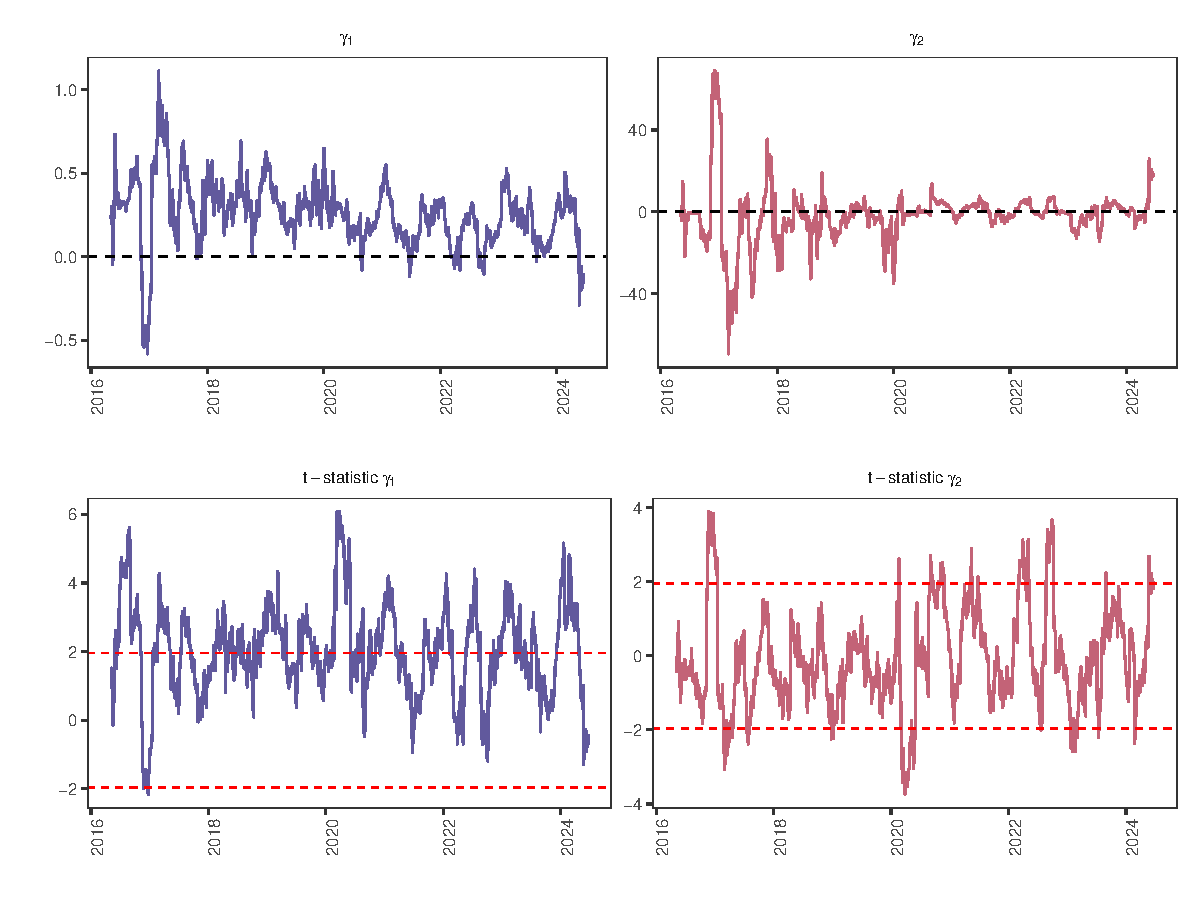
\includegraphics{alt_energy_herding_files/figure-pdf/fig-rolling_window-1.pdf}

}

\caption{\label{fig-rolling_window}Rolling window herding estimates.
Note: The red perforated lines indicates the 95\% confidence interval.}

\end{figure}%

We observe several periods of herding behaviour as reflected in the
troughs in Figure~\ref{fig-rolling_window}. The most prominent cases of
herding occur between March and May of 2020 followed by several
instances of herding in the period that extends from March through April
of 2017 (when \(\gamma_2\) averaged -45.5) and the period of
February-March of 2023 (when \(\gamma_2\) averaged -7.68).We observe
significant herding in the onset of the COVID-19 crisis 2020, which was
short lived as market adapted. The rest of the Covid period was in the
main characterised by anti-herding behaviour. \citet{ghorbel2023} and
\citet{dhall2020} found similar results. Lastly, similar to
\citet{mohamad2024} we observe no herding behaviour related to the
Russia-Ukraine war. \citet{mohamad2024} highlights the importance of
context in understanding the link between herding and market events. On
the other side, we derive significant moments of anti-herding behaviour
in the clean energy ETFs by observing the spikes in
Figure~\ref{fig-rolling_window}. Cross sectional dispersion appears to
increase with respect to market-wide returns which is a sign of
anti-herding behaviour on behalf of investors around December of 2016
and later during September of 2022.

\subsection{Climate-related uncertainty and herding
behaviour}\label{climate-related-uncertainty-and-herding-behaviour}

The behaviour of participants in energy markets is closely related to
the developments in the field of climate risks, carbon emissions and
environmentally friendly policies. In particular, following the
implementation of the Paris agreement in November 2016, climate policy
uncertainty has become in the epicenter of interest across carbon and
energy markets. There are a few studies that attempt to quantify the
effects of uncertainty related to climate on the economy and financial
markets \citep[see inter alia,][]{gabriel2024, bolton2021, krueger2020}.
To this end, \citet{bua2024} developed two climate risk related indexes
namely transition and physical risk using a text-based approach in order
to study the effect of these risks in financial markets. It is expected
that investors would prefer to hold assets that perform well in the face
of increasing climate change risks, even if this entails accepting lower
returns for such climate-hedging assets. Therefore, in the context of
our study and following previous studies that study the determinants of
herding behaviour \citep[see][]{bouri2019, demirer2018}, we attempt to
study the effect of climate-related uncertainty on the formation of
herding behavior in the clean energy market.

We use a probit model to relate herding to the two climate risk indexes
developed by \citet{bua2024} in the following manner:

\begin{equation}\phantomsection\label{eq-climate}{
Pr(D^{herd} = 1 |\lambda_0 +  \lambda_1TRI  + \lambda_2PRI) = \lambda_0 +  \lambda_1TRI  + \lambda_2PRI,
}\end{equation}

where \(D^{herd}\) takes a value of 1 during periods of statistically
significant herding (i.e., for days when the rolling t-statistic on
\(\gamma_2 < −1.96\) in Figure~\ref{fig-rolling_window}) and zero
otherwise. \(TRI\) is the transitional risk index and \(PRI\) is the
physical risk index.

The results from the Probit model are reported in
Table~\ref{tbl-probit_analysis}, where only the physical risk index
significantly decreases the probability of herding.\footnote{It should
  be noted that due to availability issues the probit analysis ends in
  December of 2023.} In other words, climate risks is good news for
clean energy stocks or firms resulting in anti-herding behaviour. This
implies that in the presence of higher physical risk with respect to the
climate, clean energy ETFs become a more attractive investment option
for investors that allocate their money to the various alternative
energy investment products. As a result, the cross-sectional dispersion
of clean energy ETFs tends to increase. Our results are in line with
those of relevant studies such as \citet{gabriel2024} who claimed that
in the event of climate policy shocks, clean energy assets could serve
the role of hedging instruments.

\global\setlength{\Oldarrayrulewidth}{\arrayrulewidth}

\global\setlength{\Oldtabcolsep}{\tabcolsep}

\setlength{\tabcolsep}{2pt}

\renewcommand*{\arraystretch}{0.7}



\providecommand{\ascline}[3]{\noalign{\global\arrayrulewidth #1}\arrayrulecolor[HTML]{#2}\cline{#3}}

\begin{longtable}[l]{|p{3.68in}|p{2.04in}}

\caption{\label{tbl-probit_analysis}Estimation results of the probit
model}

\tabularnewline

\ascline{1pt}{000000}{1-2}

\multicolumn{1}{!{\color[HTML]{FFFFFF}\vrule width 1pt}>{\raggedright}m{\dimexpr 3.68in+0\tabcolsep}}{\textcolor[HTML]{000000}{\fontsize{7}{7}\selectfont{\global\setmainfont{Arial}{Variable}}}} & \multicolumn{1}{!{\color[HTML]{FFFFFF}\vrule width 1pt}>{\centering}m{\dimexpr 2.04in+0\tabcolsep}!{\color[HTML]{FFFFFF}\vrule width 1pt}}{\textcolor[HTML]{000000}{\fontsize{7}{7}\selectfont{\global\setmainfont{Arial}{Coefficient}}}} \\

\ascline{1pt}{000000}{1-2}\endfirsthead 

\ascline{1pt}{000000}{1-2}

\multicolumn{1}{!{\color[HTML]{FFFFFF}\vrule width 1pt}>{\raggedright}m{\dimexpr 3.68in+0\tabcolsep}}{\textcolor[HTML]{000000}{\fontsize{7}{7}\selectfont{\global\setmainfont{Arial}{Variable}}}} & \multicolumn{1}{!{\color[HTML]{FFFFFF}\vrule width 1pt}>{\centering}m{\dimexpr 2.04in+0\tabcolsep}!{\color[HTML]{FFFFFF}\vrule width 1pt}}{\textcolor[HTML]{000000}{\fontsize{7}{7}\selectfont{\global\setmainfont{Arial}{Coefficient}}}} \\

\ascline{1pt}{000000}{1-2}\endhead



\multicolumn{1}{!{\color[HTML]{FFFFFF}\vrule width 1pt}>{\raggedright}m{\dimexpr 3.68in+0\tabcolsep}}{\textcolor[HTML]{000000}{\fontsize{7}{7}\selectfont{\global\setmainfont{Arial}{$\lambda_0$}}}} & \multicolumn{1}{!{\color[HTML]{FFFFFF}\vrule width 1pt}>{\centering}m{\dimexpr 2.04in+0\tabcolsep}!{\color[HTML]{FFFFFF}\vrule width 1pt}}{\textcolor[HTML]{000000}{\fontsize{7}{7}\selectfont{\global\setmainfont{Arial}{\ -1.506***}}}} \\

\ascline{1pt}{FFFFFF}{1-2}



\multicolumn{1}{!{\color[HTML]{FFFFFF}\vrule width 1pt}>{\raggedright}m{\dimexpr 3.68in+0\tabcolsep}}{\textcolor[HTML]{000000}{\fontsize{7}{7}\selectfont{\global\setmainfont{Arial}{$\lambda_1$}}}} & \multicolumn{1}{!{\color[HTML]{FFFFFF}\vrule width 1pt}>{\centering}m{\dimexpr 2.04in+0\tabcolsep}!{\color[HTML]{FFFFFF}\vrule width 1pt}}{\textcolor[HTML]{000000}{\fontsize{7}{7}\selectfont{\global\setmainfont{Arial}{-4.607***}}}} \\

\ascline{1pt}{FFFFFF}{1-2}



\multicolumn{1}{!{\color[HTML]{FFFFFF}\vrule width 1pt}>{\raggedright}m{\dimexpr 3.68in+0\tabcolsep}}{\textcolor[HTML]{000000}{\fontsize{7}{7}\selectfont{\global\setmainfont{Arial}{$\lambda_2$}}}} & \multicolumn{1}{!{\color[HTML]{FFFFFF}\vrule width 1pt}>{\centering}m{\dimexpr 2.04in+0\tabcolsep}!{\color[HTML]{FFFFFF}\vrule width 1pt}}{\textcolor[HTML]{000000}{\fontsize{7}{7}\selectfont{\global\setmainfont{Arial}{-1.318}}}} \\

\ascline{1pt}{000000}{1-2}



\multicolumn{1}{!{\color[HTML]{FFFFFF}\vrule width 1pt}>{\raggedright}m{\dimexpr 3.68in+0\tabcolsep}}{\textcolor[HTML]{000000}{\fontsize{7}{7}\selectfont{\global\setmainfont{Arial}{Log\ Likelihood}}}} & \multicolumn{1}{!{\color[HTML]{FFFFFF}\vrule width 1pt}>{\centering}m{\dimexpr 2.04in+0\tabcolsep}!{\color[HTML]{FFFFFF}\vrule width 1pt}}{\textcolor[HTML]{000000}{\fontsize{7}{7}\selectfont{\global\setmainfont{Arial}{-484.7}}}} \\

\ascline{1pt}{FFFFFF}{1-2}



\multicolumn{1}{!{\color[HTML]{FFFFFF}\vrule width 1pt}>{\raggedright}m{\dimexpr 3.68in+0\tabcolsep}}{\textcolor[HTML]{000000}{\fontsize{7}{7}\selectfont{\global\setmainfont{Arial}{Observations\ with\ Dependent\ Variable\ (Dep)\ =\ 0}}}} & \multicolumn{1}{!{\color[HTML]{FFFFFF}\vrule width 1pt}>{\centering}m{\dimexpr 2.04in+0\tabcolsep}!{\color[HTML]{FFFFFF}\vrule width 1pt}}{\textcolor[HTML]{000000}{\fontsize{7}{7}\selectfont{\global\setmainfont{Arial}{1816}}}} \\

\ascline{1pt}{FFFFFF}{1-2}



\multicolumn{1}{!{\color[HTML]{FFFFFF}\vrule width 1pt}>{\raggedright}m{\dimexpr 3.68in+0\tabcolsep}}{\textcolor[HTML]{000000}{\fontsize{7}{7}\selectfont{\global\setmainfont{Arial}{Observations\ with\ Dependent\ Variable\ (Dep)\ =\ 1}}}} & \multicolumn{1}{!{\color[HTML]{FFFFFF}\vrule width 1pt}>{\centering}m{\dimexpr 2.04in+0\tabcolsep}!{\color[HTML]{FFFFFF}\vrule width 1pt}}{\textcolor[HTML]{000000}{\fontsize{7}{7}\selectfont{\global\setmainfont{Arial}{134}}}} \\

\ascline{1pt}{000000}{1-2}



\multicolumn{2}{>{\raggedright}m{\dimexpr 5.72in+2\tabcolsep}}{\textcolor[HTML]{000000}{\fontsize{7}{7}\selectfont{\global\setmainfont{Arial}{Notes:\ **,***\ denotes\ statistically\ significant\ at\ 5\%\ and\ 1\%}}}} \\

\ascline{1pt}{000000}{1-2}


\end{longtable}

\arrayrulecolor[HTML]{000000}

\global\setlength{\arrayrulewidth}{\Oldarrayrulewidth}

\global\setlength{\tabcolsep}{\Oldtabcolsep}

\renewcommand*{\arraystretch}{1}

Furthermore, we develop two additional models to study the effect of
climate risks on herding behaviour. We split the sample into two groups
based on the median value of the TRI and PRI. We then estimate the
following two models:

\begin{equation}\phantomsection\label{eq-climate_high}{
Pr(D^{herd} = 1 |\lambda_0 +\lambda_1D^{TRI}_{high}TRI + \lambda_2D^{PRI}_{high}PRI) = \lambda_0 +\lambda_1D^{TRI}_{high}TRI + \lambda_2D^{PRI}_{high}PRI, and
}\end{equation}

\begin{equation}\phantomsection\label{eq-climate_low}{
Pr(D^{herd} = 1 |\lambda_0 +\lambda_1D^{TRI}_{low}TRI + \lambda_2D^{PRI}_{low}PRI) = \lambda_0 +\lambda_1D^{TRI}_{low}TRI + \lambda_2D^{PRI}_{low}PRI, 
}\end{equation}

where \(D^{herd}\) is the same as in Equation~\ref{eq-climate}.
\(D^{TRI}_{high}\) and \(D^{PRI}_{high}\) are dummy variables that take
a value of 1 if the value of the TRI and PRI are above the median and
zero otherwise. Similarly, \(D^{TRI}_{low}\) and \(D^{PRI}_{low}\) are
dummy variables that take a value of 1 if the value of the TRI and PRI
are below the median and zero otherwise.

\global\setlength{\Oldarrayrulewidth}{\arrayrulewidth}

\global\setlength{\Oldtabcolsep}{\tabcolsep}

\setlength{\tabcolsep}{2pt}

\renewcommand*{\arraystretch}{0.7}



\providecommand{\ascline}[3]{\noalign{\global\arrayrulewidth #1}\arrayrulecolor[HTML]{#2}\cline{#3}}

\begin{longtable}[l]{|p{2.59in}|p{1.90in}|p{1.86in}}

\caption{\label{tbl-probit_analysis2}Estimation results of the probit
model with high and low climate risk indexes (above or below median)}

\tabularnewline

\ascline{1pt}{000000}{1-3}

\multicolumn{1}{!{\color[HTML]{FFFFFF}\vrule width 1pt}>{\raggedright}m{\dimexpr 2.59in+0\tabcolsep}}{\textcolor[HTML]{000000}{\fontsize{7}{7}\selectfont{\global\setmainfont{Arial}{\ }}}} & \multicolumn{1}{!{\color[HTML]{FFFFFF}\vrule width 1pt}>{\centering}m{\dimexpr 1.9in+0\tabcolsep}}{\textcolor[HTML]{000000}{\fontsize{7}{7}\selectfont{\global\setmainfont{Arial}{High}}}} & \multicolumn{1}{!{\color[HTML]{FFFFFF}\vrule width 1pt}>{\centering}m{\dimexpr 1.86in+0\tabcolsep}!{\color[HTML]{FFFFFF}\vrule width 1pt}}{\textcolor[HTML]{000000}{\fontsize{7}{7}\selectfont{\global\setmainfont{Arial}{Low}}}} \\

\ascline{1pt}{000000}{1-3}\endfirsthead 

\ascline{1pt}{000000}{1-3}

\multicolumn{1}{!{\color[HTML]{FFFFFF}\vrule width 1pt}>{\raggedright}m{\dimexpr 2.59in+0\tabcolsep}}{\textcolor[HTML]{000000}{\fontsize{7}{7}\selectfont{\global\setmainfont{Arial}{\ }}}} & \multicolumn{1}{!{\color[HTML]{FFFFFF}\vrule width 1pt}>{\centering}m{\dimexpr 1.9in+0\tabcolsep}}{\textcolor[HTML]{000000}{\fontsize{7}{7}\selectfont{\global\setmainfont{Arial}{High}}}} & \multicolumn{1}{!{\color[HTML]{FFFFFF}\vrule width 1pt}>{\centering}m{\dimexpr 1.86in+0\tabcolsep}!{\color[HTML]{FFFFFF}\vrule width 1pt}}{\textcolor[HTML]{000000}{\fontsize{7}{7}\selectfont{\global\setmainfont{Arial}{Low}}}} \\

\ascline{1pt}{000000}{1-3}\endhead



\multicolumn{1}{!{\color[HTML]{FFFFFF}\vrule width 1pt}>{\raggedright}m{\dimexpr 2.59in+0\tabcolsep}}{\textcolor[HTML]{000000}{\fontsize{7}{7}\selectfont{\global\setmainfont{Arial}{$\lambda_1$}}}} & \multicolumn{1}{!{\color[HTML]{FFFFFF}\vrule width 1pt}>{\centering}m{\dimexpr 1.9in+0\tabcolsep}}{\textcolor[HTML]{000000}{\fontsize{7}{7}\selectfont{\global\setmainfont{Arial}{-6.736*}}}} & \multicolumn{1}{!{\color[HTML]{FFFFFF}\vrule width 1pt}>{\centering}m{\dimexpr 1.86in+0\tabcolsep}!{\color[HTML]{FFFFFF}\vrule width 1pt}}{\textcolor[HTML]{000000}{\fontsize{7}{7}\selectfont{\global\setmainfont{Arial}{-6.118}}}} \\

\ascline{1pt}{FFFFFF}{1-3}



\multicolumn{1}{!{\color[HTML]{FFFFFF}\vrule width 1pt}>{\raggedright}m{\dimexpr 2.59in+0\tabcolsep}}{\textcolor[HTML]{000000}{\fontsize{7}{7}\selectfont{\global\setmainfont{Arial}{$\lambda_2$}}}} & \multicolumn{1}{!{\color[HTML]{FFFFFF}\vrule width 1pt}>{\centering}m{\dimexpr 1.9in+0\tabcolsep}}{\textcolor[HTML]{000000}{\fontsize{7}{7}\selectfont{\global\setmainfont{Arial}{-1.798}}}} & \multicolumn{1}{!{\color[HTML]{FFFFFF}\vrule width 1pt}>{\centering}m{\dimexpr 1.86in+0\tabcolsep}!{\color[HTML]{FFFFFF}\vrule width 1pt}}{\textcolor[HTML]{000000}{\fontsize{7}{7}\selectfont{\global\setmainfont{Arial}{-2.581}}}} \\

\ascline{1pt}{000000}{1-3}



\multicolumn{3}{>{\raggedright}m{\dimexpr 6.34in+4\tabcolsep}}{\textcolor[HTML]{000000}{\fontsize{7}{7}\selectfont{\global\setmainfont{Arial}{Notes:\ *,\ denotes\ statistically\ significant\ at\ 10\%}}}} \\

\ascline{1pt}{000000}{1-3}


\end{longtable}

\arrayrulecolor[HTML]{000000}

\global\setlength{\arrayrulewidth}{\Oldarrayrulewidth}

\global\setlength{\tabcolsep}{\Oldtabcolsep}

\renewcommand*{\arraystretch}{1}

We use these high PRI and high TRI in one probit regression and low TRI
and low PRI in another. Results are presented in
Table~\ref{tbl-probit_analysis2}. We observe higher uncertainty that
stems from physical or transition risk causes anti-herding which is in
line with the logic we discussed earlier.

\section{Conclusion}\label{conclusion}

This study offers novel and valuable insights into herding behaviour in
clean energy ETFs. We used various herding behaviour tests to achieve
this. First, the baseline herding tests revealed significant evidence of
herding behaviour. Second, the asymmetric herding tests showed that
herding behaviour was present in both bear and bull markets. Lastly, the
results of the time-varying tests point to significant periodic herding.
However, the results further indicate that herding in US clean energy
ETFs was not mainly related to climate-related risks or uncertainty. The
probit analysis showed that climate-related uncertainty reduced the
probability of herding or led to investor anti-herding behaviour. We
differ to the literature on the factors that drive herding in these ETFs
\citep[for example,][]{loang2023, koutmos2024, przychodzen2016}. Our
results, similar to \citet{bua2024}, indicate that investors did not
herd on climate-related uncertainty, and sought returns whilst hedging
against climate-related risk. This is a positive for the financial
stability of these growing alternative investment indices.

\newpage

\section*{References}\label{references}
\addcontentsline{toc}{section}{References}

\renewcommand{\bibsection}{}
\bibliography{energy_herding.bib}

\setcounter{section}{0}
\renewcommand{\thesection}{\Alph{section}}

\setcounter{table}{0}
\renewcommand{\thetable}{A\arabic{table}}

\setcounter{figure}{0}
\renewcommand{\thefigure}{A\arabic{figure}}

\newpage

\section{Appendix}\label{appendix}

\subsection{ETFs used in the study}\label{etfs-used-in-the-study}

\global\setlength{\Oldarrayrulewidth}{\arrayrulewidth}

\global\setlength{\Oldtabcolsep}{\tabcolsep}

\setlength{\tabcolsep}{2pt}

\renewcommand*{\arraystretch}{0.7}



\providecommand{\ascline}[3]{\noalign{\global\arrayrulewidth #1}\arrayrulecolor[HTML]{#2}\cline{#3}}

\begin{longtable}[l]{|p{5.39in}}

\caption{\label{tbl-data}List of green ETFs used in the study}

\tabularnewline

\ascline{1pt}{000000}{1-1}

\multicolumn{1}{!{\color[HTML]{FFFFFF}\vrule width 1pt}>{\raggedright}m{\dimexpr 5.39in+0\tabcolsep}!{\color[HTML]{FFFFFF}\vrule width 1pt}}{\textcolor[HTML]{000000}{\fontsize{7}{7}\selectfont{\global\setmainfont{Arial}{ETF}}}} \\

\ascline{1pt}{000000}{1-1}\endfirsthead 

\ascline{1pt}{000000}{1-1}

\multicolumn{1}{!{\color[HTML]{FFFFFF}\vrule width 1pt}>{\raggedright}m{\dimexpr 5.39in+0\tabcolsep}!{\color[HTML]{FFFFFF}\vrule width 1pt}}{\textcolor[HTML]{000000}{\fontsize{7}{7}\selectfont{\global\setmainfont{Arial}{ETF}}}} \\

\ascline{1pt}{000000}{1-1}\endhead



\multicolumn{1}{!{\color[HTML]{FFFFFF}\vrule width 1pt}>{\raggedright}m{\dimexpr 5.39in+0\tabcolsep}!{\color[HTML]{FFFFFF}\vrule width 1pt}}{\textcolor[HTML]{000000}{\fontsize{7}{7}\selectfont{\global\setmainfont{Arial}{ALPS\ CLEAN\ ENERGY\ ETF}}}} \\

\ascline{1pt}{FFFFFF}{1-1}



\multicolumn{1}{!{\color[HTML]{FFFFFF}\vrule width 1pt}>{\raggedright}m{\dimexpr 5.39in+0\tabcolsep}!{\color[HTML]{FFFFFF}\vrule width 1pt}}{\textcolor[HTML]{000000}{\fontsize{7}{7}\selectfont{\global\setmainfont{Arial}{BLUE\ HORIZON\ BNE\ ETF}}}} \\

\ascline{1pt}{FFFFFF}{1-1}



\multicolumn{1}{!{\color[HTML]{FFFFFF}\vrule width 1pt}>{\raggedright}m{\dimexpr 5.39in+0\tabcolsep}!{\color[HTML]{FFFFFF}\vrule width 1pt}}{\textcolor[HTML]{000000}{\fontsize{7}{7}\selectfont{\global\setmainfont{Arial}{SPDR\ S\&P\ KENSHO\ CLEAN\ POWER\ ETF}}}} \\

\ascline{1pt}{FFFFFF}{1-1}



\multicolumn{1}{!{\color[HTML]{FFFFFF}\vrule width 1pt}>{\raggedright}m{\dimexpr 5.39in+0\tabcolsep}!{\color[HTML]{FFFFFF}\vrule width 1pt}}{\textcolor[HTML]{000000}{\fontsize{7}{7}\selectfont{\global\setmainfont{Arial}{GLOBAL\ X\ CLEANTECH\ ETF}}}} \\

\ascline{1pt}{FFFFFF}{1-1}



\multicolumn{1}{!{\color[HTML]{FFFFFF}\vrule width 1pt}>{\raggedright}m{\dimexpr 5.39in+0\tabcolsep}!{\color[HTML]{FFFFFF}\vrule width 1pt}}{\textcolor[HTML]{000000}{\fontsize{7}{7}\selectfont{\global\setmainfont{Arial}{PROSHARES\ S\&P\ KENSHO\ CLEANTECH\ ETF}}}} \\

\ascline{1pt}{FFFFFF}{1-1}



\multicolumn{1}{!{\color[HTML]{FFFFFF}\vrule width 1pt}>{\raggedright}m{\dimexpr 5.39in+0\tabcolsep}!{\color[HTML]{FFFFFF}\vrule width 1pt}}{\textcolor[HTML]{000000}{\fontsize{7}{7}\selectfont{\global\setmainfont{Arial}{INVESCO\ MSCI\ SUSTAINABLE\ FUTURE\ ETF}}}} \\

\ascline{1pt}{FFFFFF}{1-1}



\multicolumn{1}{!{\color[HTML]{FFFFFF}\vrule width 1pt}>{\raggedright}m{\dimexpr 5.39in+0\tabcolsep}!{\color[HTML]{FFFFFF}\vrule width 1pt}}{\textcolor[HTML]{000000}{\fontsize{7}{7}\selectfont{\global\setmainfont{Arial}{FIRST\ TRUST\ GLOBAL\ WIND\ ENERGY\ ETF}}}} \\

\ascline{1pt}{FFFFFF}{1-1}



\multicolumn{1}{!{\color[HTML]{FFFFFF}\vrule width 1pt}>{\raggedright}m{\dimexpr 5.39in+0\tabcolsep}!{\color[HTML]{FFFFFF}\vrule width 1pt}}{\textcolor[HTML]{000000}{\fontsize{7}{7}\selectfont{\global\setmainfont{Arial}{FIDELITY\ CLEAN\ ENERGY\ ETF}}}} \\

\ascline{1pt}{FFFFFF}{1-1}



\multicolumn{1}{!{\color[HTML]{FFFFFF}\vrule width 1pt}>{\raggedright}m{\dimexpr 5.39in+0\tabcolsep}!{\color[HTML]{FFFFFF}\vrule width 1pt}}{\textcolor[HTML]{000000}{\fontsize{7}{7}\selectfont{\global\setmainfont{Arial}{GLDS.BLOOMBERG\ CN.\ EN.\ EQ.ETF}}}} \\

\ascline{1pt}{FFFFFF}{1-1}



\multicolumn{1}{!{\color[HTML]{FFFFFF}\vrule width 1pt}>{\raggedright}m{\dimexpr 5.39in+0\tabcolsep}!{\color[HTML]{FFFFFF}\vrule width 1pt}}{\textcolor[HTML]{000000}{\fontsize{7}{7}\selectfont{\global\setmainfont{Arial}{FST.NQ.CN.EDGE\ SMRT.GRID\ INFRA\ IDX\ ETF}}}} \\

\ascline{1pt}{FFFFFF}{1-1}



\multicolumn{1}{!{\color[HTML]{FFFFFF}\vrule width 1pt}>{\raggedright}m{\dimexpr 5.39in+0\tabcolsep}!{\color[HTML]{FFFFFF}\vrule width 1pt}}{\textcolor[HTML]{000000}{\fontsize{7}{7}\selectfont{\global\setmainfont{Arial}{DEFIANCE\ NEXT\ GEN\ H2\ ETF}}}} \\

\ascline{1pt}{FFFFFF}{1-1}



\multicolumn{1}{!{\color[HTML]{FFFFFF}\vrule width 1pt}>{\raggedright}m{\dimexpr 5.39in+0\tabcolsep}!{\color[HTML]{FFFFFF}\vrule width 1pt}}{\textcolor[HTML]{000000}{\fontsize{7}{7}\selectfont{\global\setmainfont{Arial}{DIREXION\ HYDROGEN\ ETF}}}} \\

\ascline{1pt}{FFFFFF}{1-1}



\multicolumn{1}{!{\color[HTML]{FFFFFF}\vrule width 1pt}>{\raggedright}m{\dimexpr 5.39in+0\tabcolsep}!{\color[HTML]{FFFFFF}\vrule width 1pt}}{\textcolor[HTML]{000000}{\fontsize{7}{7}\selectfont{\global\setmainfont{Arial}{GLOBAL\ X\ HYDROGEN\ ETF}}}} \\

\ascline{1pt}{FFFFFF}{1-1}



\multicolumn{1}{!{\color[HTML]{FFFFFF}\vrule width 1pt}>{\raggedright}m{\dimexpr 5.39in+0\tabcolsep}!{\color[HTML]{FFFFFF}\vrule width 1pt}}{\textcolor[HTML]{000000}{\fontsize{7}{7}\selectfont{\global\setmainfont{Arial}{ISHARES\ GLOBAL\ CLEAN\ EN.\ ETF}}}} \\

\ascline{1pt}{FFFFFF}{1-1}



\multicolumn{1}{!{\color[HTML]{FFFFFF}\vrule width 1pt}>{\raggedright}m{\dimexpr 5.39in+0\tabcolsep}!{\color[HTML]{FFFFFF}\vrule width 1pt}}{\textcolor[HTML]{000000}{\fontsize{7}{7}\selectfont{\global\setmainfont{Arial}{BLACKR.WLD.EXUS\ CRBN\ TSTN.READINESS}}}} \\

\ascline{1pt}{FFFFFF}{1-1}



\multicolumn{1}{!{\color[HTML]{FFFFFF}\vrule width 1pt}>{\raggedright}m{\dimexpr 5.39in+0\tabcolsep}!{\color[HTML]{FFFFFF}\vrule width 1pt}}{\textcolor[HTML]{000000}{\fontsize{7}{7}\selectfont{\global\setmainfont{Arial}{NUB.CBN.TSTN.\&\ INFRA}}}} \\

\ascline{1pt}{FFFFFF}{1-1}



\multicolumn{1}{!{\color[HTML]{FFFFFF}\vrule width 1pt}>{\raggedright}m{\dimexpr 5.39in+0\tabcolsep}!{\color[HTML]{FFFFFF}\vrule width 1pt}}{\textcolor[HTML]{000000}{\fontsize{7}{7}\selectfont{\global\setmainfont{Arial}{TCW\ TRANSFORM\ SYSTEMS\ ETF}}}} \\

\ascline{1pt}{FFFFFF}{1-1}



\multicolumn{1}{!{\color[HTML]{FFFFFF}\vrule width 1pt}>{\raggedright}m{\dimexpr 5.39in+0\tabcolsep}!{\color[HTML]{FFFFFF}\vrule width 1pt}}{\textcolor[HTML]{000000}{\fontsize{7}{7}\selectfont{\global\setmainfont{Arial}{VANECK\ URANIUM\ AND\ NUCLEAR\ ENERGY}}}} \\

\ascline{1pt}{FFFFFF}{1-1}



\multicolumn{1}{!{\color[HTML]{FFFFFF}\vrule width 1pt}>{\raggedright}m{\dimexpr 5.39in+0\tabcolsep}!{\color[HTML]{FFFFFF}\vrule width 1pt}}{\textcolor[HTML]{000000}{\fontsize{7}{7}\selectfont{\global\setmainfont{Arial}{NUVEEN\ GLOBAL\ NET\ ZERO\ TRANSITION\ ETF}}}} \\

\ascline{1pt}{FFFFFF}{1-1}



\multicolumn{1}{!{\color[HTML]{FFFFFF}\vrule width 1pt}>{\raggedright}m{\dimexpr 5.39in+0\tabcolsep}!{\color[HTML]{FFFFFF}\vrule width 1pt}}{\textcolor[HTML]{000000}{\fontsize{7}{7}\selectfont{\global\setmainfont{Arial}{SPDR\ MSCI\ USA\ CIM.\ PA.\ ALIGNED\ ETF}}}} \\

\ascline{1pt}{FFFFFF}{1-1}



\multicolumn{1}{!{\color[HTML]{FFFFFF}\vrule width 1pt}>{\raggedright}m{\dimexpr 5.39in+0\tabcolsep}!{\color[HTML]{FFFFFF}\vrule width 1pt}}{\textcolor[HTML]{000000}{\fontsize{7}{7}\selectfont{\global\setmainfont{Arial}{INVESCO\ GLOBAL\ CLEAN\ ENERGY\ ETF}}}} \\

\ascline{1pt}{FFFFFF}{1-1}



\multicolumn{1}{!{\color[HTML]{FFFFFF}\vrule width 1pt}>{\raggedright}m{\dimexpr 5.39in+0\tabcolsep}!{\color[HTML]{FFFFFF}\vrule width 1pt}}{\textcolor[HTML]{000000}{\fontsize{7}{7}\selectfont{\global\setmainfont{Arial}{FST.NQ.CN.EDGE\ GREY.ETF}}}} \\

\ascline{1pt}{FFFFFF}{1-1}



\multicolumn{1}{!{\color[HTML]{FFFFFF}\vrule width 1pt}>{\raggedright}m{\dimexpr 5.39in+0\tabcolsep}!{\color[HTML]{FFFFFF}\vrule width 1pt}}{\textcolor[HTML]{000000}{\fontsize{7}{7}\selectfont{\global\setmainfont{Arial}{GLOBAL\ X\ SOLAR\ ETF}}}} \\

\ascline{1pt}{FFFFFF}{1-1}



\multicolumn{1}{!{\color[HTML]{FFFFFF}\vrule width 1pt}>{\raggedright}m{\dimexpr 5.39in+0\tabcolsep}!{\color[HTML]{FFFFFF}\vrule width 1pt}}{\textcolor[HTML]{000000}{\fontsize{7}{7}\selectfont{\global\setmainfont{Arial}{GLOBAL\ X\ RENEWABLE\ ENERGY\ PRODUCERS}}}} \\

\ascline{1pt}{FFFFFF}{1-1}



\multicolumn{1}{!{\color[HTML]{FFFFFF}\vrule width 1pt}>{\raggedright}m{\dimexpr 5.39in+0\tabcolsep}!{\color[HTML]{FFFFFF}\vrule width 1pt}}{\textcolor[HTML]{000000}{\fontsize{7}{7}\selectfont{\global\setmainfont{Arial}{TRUESHARES\ EAG.GLB.\ RENWEN.ETF}}}} \\

\ascline{1pt}{FFFFFF}{1-1}



\multicolumn{1}{!{\color[HTML]{FFFFFF}\vrule width 1pt}>{\raggedright}m{\dimexpr 5.39in+0\tabcolsep}!{\color[HTML]{FFFFFF}\vrule width 1pt}}{\textcolor[HTML]{000000}{\fontsize{7}{7}\selectfont{\global\setmainfont{Arial}{VANECK\ LOW\ CARBON\ ENERGY\ ETF}}}} \\

\ascline{1pt}{FFFFFF}{1-1}



\multicolumn{1}{!{\color[HTML]{FFFFFF}\vrule width 1pt}>{\raggedright}m{\dimexpr 5.39in+0\tabcolsep}!{\color[HTML]{FFFFFF}\vrule width 1pt}}{\textcolor[HTML]{000000}{\fontsize{7}{7}\selectfont{\global\setmainfont{Arial}{SMARTETFS\ SUST.EN.\ II\ ETF}}}} \\

\ascline{1pt}{FFFFFF}{1-1}



\multicolumn{1}{!{\color[HTML]{FFFFFF}\vrule width 1pt}>{\raggedright}m{\dimexpr 5.39in+0\tabcolsep}!{\color[HTML]{FFFFFF}\vrule width 1pt}}{\textcolor[HTML]{000000}{\fontsize{7}{7}\selectfont{\global\setmainfont{Arial}{INVESCO\ SOLAR\ ETF}}}} \\

\ascline{1pt}{FFFFFF}{1-1}



\multicolumn{1}{!{\color[HTML]{FFFFFF}\vrule width 1pt}>{\raggedright}m{\dimexpr 5.39in+0\tabcolsep}!{\color[HTML]{FFFFFF}\vrule width 1pt}}{\textcolor[HTML]{000000}{\fontsize{7}{7}\selectfont{\global\setmainfont{Arial}{VIRTUS\ DUFF\ \&\ PHELPS\ CLEAN\ ENERGY\ ETF}}}} \\

\ascline{1pt}{FFFFFF}{1-1}



\multicolumn{1}{!{\color[HTML]{FFFFFF}\vrule width 1pt}>{\raggedright}m{\dimexpr 5.39in+0\tabcolsep}!{\color[HTML]{FFFFFF}\vrule width 1pt}}{\textcolor[HTML]{000000}{\fontsize{7}{7}\selectfont{\global\setmainfont{Arial}{GLOBAL\ X\ WIND\ ENERGY\ ETF}}}} \\

\ascline{1pt}{000000}{1-1}



\multicolumn{1}{>{\raggedright}m{\dimexpr 5.39in+0\tabcolsep}}{\textcolor[HTML]{000000}{\fontsize{7}{7}\selectfont{\global\setmainfont{Arial}{Note:\ Details\ on\ these\ funds\ can\ be\ found\ on\ Yahoo\ Finance.}}}} \\




\end{longtable}

\arrayrulecolor[HTML]{000000}

\global\setlength{\arrayrulewidth}{\Oldarrayrulewidth}

\global\setlength{\tabcolsep}{\Oldtabcolsep}

\renewcommand*{\arraystretch}{1}





\end{document}
